\documentclass[conference]{IEEEtran}
\usepackage{cite}
\usepackage{amsmath,amssymb,amsfonts}
\usepackage{algorithmic}
\usepackage{graphicx}
\usepackage{textcomp}
\usepackage{xcolor}
\usepackage{booktabs}
\usepackage{multirow}
\usepackage{hyperref}
\usepackage{float}
\usepackage{array}
\usepackage{tabularx}
\usepackage{caption}
\usepackage{subcaption}

\def\BibTeX{{\rm B\kern-.05em{\sc i\kern-.025em b}\kern-.08em
    T\kern-.1667em\lower.7ex\hbox{E}\kern-.125emX}}

\begin{document}

\title{Customer Segmentation and Clustering in Banking Using Data Mining Techniques: A Comparative Study}

\author{
\IEEEauthorblockN{Ruchit Doshi}
\IEEEauthorblockA{\textit{Department of Computer Engineering}\\
\textit{Marwadi University}\\
Rajkot, Gujarat, India}
\and
\IEEEauthorblockN{Rudrasinh Revar}
\IEEEauthorblockA{\textit{Department of Computer Engineering}\\
\textit{Marwadi University}\\
Rajkot, Gujarat, India}
\and
\IEEEauthorblockN{Aditya Mevcha}
\IEEEauthorblockA{\textit{Department of Computer Engineering}\\
\textit{Marwadi University}\\
Rajkot, Gujarat, India}
\and
\IEEEauthorblockN{Krutarth Gadhiya}
\IEEEauthorblockA{\textit{Department of Computer Engineering}\\
\textit{Marwadi University}\\
Rajkot, Gujarat, India}
\and
\IEEEauthorblockN{Rudra Mehta}
\IEEEauthorblockA{\textit{Department of Computer Engineering}\\
\textit{Marwadi University}\\
Rajkot, Gujarat, India}
\and
\IEEEauthorblockN{Sahir Suma}
\IEEEauthorblockA{\textit{Department of Computer Engineering}\\
\textit{Marwadi University}\\
Rajkot, Gujarat, India}
}

\maketitle

\begin{abstract}
The banking industry generates vast volumes of transactional and behavioral data, which create opportunities for understanding customers and for detecting fraudulent activity. This paper presents a comparative study of eight data mining algorithms applied to two banking problems: customer segmentation and fraud detection. For segmentation, K-Means, Hierarchical (Agglomerative) Clustering, DBSCAN, and Gaussian Mixture Models (GMM) are evaluated on the CC GENERAL credit card behavioral dataset, which describes 8,950 customers through 17 behavioral variables, using the Silhouette Score, the Davies-Bouldin Index, and the Calinski-Harabasz Index. For fraud detection, Logistic Regression, Random Forest, Isolation Forest, and XGBoost are benchmarked on the first 20,000 transactions of the European credit card fraud dataset (85 fraudulent cases) using six evaluation metrics, including ROC-AUC and Average Precision. The results show that K-Means with three clusters provides the most actionable segmentation (Silhouette Score of 0.2376 and Calinski-Harabasz Index of 2846.26) and yields three interpretable customer profiles, whereas DBSCAN attains the highest Silhouette Score (0.3707) but produces only two clusters and labels 8.1\% of customers as noise. XGBoost delivers the strongest fraud detection performance (ROC-AUC of 1.000, F1-Score of 0.971, and recall of 1.000 on the 17 fraudulent test transactions), followed by Random Forest (F1-Score of 0.882). The discussion relates these findings to the reviewed literature, acknowledges the statistical limits imposed by a small positive class, and provides guidance on algorithm selection for banking applications.
\end{abstract}

\begin{IEEEkeywords}
Data mining, customer segmentation, fraud detection, K-Means clustering, XGBoost, DBSCAN, Random Forest, Isolation Forest, banking analytics, machine learning
\end{IEEEkeywords}

% ============================================================================
%  I. INTRODUCTION
% ============================================================================
\section{Introduction}

The modern banking ecosystem is characterized by an exponential growth in digital transactions, and every card payment, balance enquiry, cash withdrawal, and repayment leaves a behavioral trace that a financial institution can store and analyze. The same digitization that enables this wealth of data also exposes banks and their customers to financial crime: worldwide card fraud losses reached approximately USD 33.83 billion in 2023 \cite{nilson2023}, which underlines the need for intelligent, automated detection systems. At the same time, banks operate in highly competitive markets in which customers expect products, pricing, and communication that reflect their individual needs. Understanding who the customers are, how they use their accounts and cards, and which of them are most valuable has therefore become a central objective of customer relationship management (CRM) \cite{ngai2011application}.

Data mining, defined as the process of discovering patterns and extracting knowledge from large datasets \cite{han2011data}, offers a coherent set of techniques for both challenges. Customer segmentation relies mainly on unsupervised learning to divide a heterogeneous customer base into internally homogeneous groups, so that marketing, credit, and service decisions can be tailored to each group instead of being applied uniformly. Fraud detection, in contrast, relies on supervised classification and anomaly detection to separate a very small number of illegitimate transactions from a very large number of legitimate ones \cite{bolton2002statistical}. Although the two tasks have different objectives, both depend on the same raw material, namely customer and transaction records, and both are sensitive to the same data quality issues such as skewed distributions, extreme values, and heterogeneous feature scales.

The importance of segmentation in banking has been documented from several directions. Systematic and state-of-the-art reviews describe supervised, unsupervised, and hybrid segmentation techniques and organize the methods used for personalized customer targeting \cite{das2022,gomes2023}. A survey focused specifically on banks reviews the data mining techniques applied to customer analysis, with emphasis on customer relationship management and customer value \cite{hasheminejad2018}. Early banking studies already showed that clustering recency, frequency, and monetary (RFM) indicators with K-Means, followed by a second partitioning using demographic attributes and a lifetime-value profile, can structure a bank's market into actionable groups \cite{kumar2012}. Later case studies on Iranian, Indonesian, and Azerbaijani banks confirmed the value of RFM-based K-Means segmentation for internet and electronic banking customers \cite{fouladifar2016,aryuni2018,aliyev2020}, and an extension of RFM with a balance dimension (RFM+B) was proposed for bank customer segmentation \cite{firdaus2021}. The same combination of RFM variables and centroid-based clustering has also been adopted in online retail, e-commerce, and food service settings \cite{singh2023,kc2026,hasugian2026}, which illustrates that the methodology generalizes beyond banking.

Credit card behavioral data have received particular attention because they combine balances, purchases, cash advances, credit limits, and repayment patterns in a compact feature set. The Elbow method has been integrated with K-Means to select the number of customer profile clusters \cite{syakur2018integration}, K-Means has been applied directly to account balance, purchase, and cash advance attributes for targeted marketing in banking \cite{gopalakrishnan2024}, and the Elbow and Silhouette criteria have been used to derive five segments of bank consumers for artificial intelligence marketing \cite{raiter2021}. Beyond K-Means, advanced data mining pipelines combining K-Means with agglomerative clustering have been used to derive customer profiles from rich demographic and purchase data \cite{sinap2025}. Hierarchical and density-oriented alternatives have likewise been explored for bank customers, including Ward linkage, BIRCH, and improved DBSCAN variants \cite{zakrzewska2005clustering,hassan2018,kikoria2020,yan2025}.

Segmentation research in banking has also broadened in terms of the evidence used to form groups. Cluster analysis has been combined with an ethical perspective on how customers are grouped \cite{kumar2024}, hybrid models have been used to estimate the propensity of customers to adopt online banking \cite{ganar2022}, two-stage clustering of survey data has been used to explore investment patterns of retail banking customers \cite{kovacs2021}, and attitude-based and emotion-based segmentations have shown that psychological variables separate customers in ways that transactions alone cannot \cite{swissvn2019,calvoporral2020}. Time-series clustering and deep sequence models extend segmentation to the temporal dynamics of behavior \cite{abbasimehr2021,barkhordar2021}, intelligent pipelines and vector embeddings automate feature engineering for risk-based and analyst-oriented segmentation \cite{zand2020,mousaeirad2020}, and churn prediction frameworks based on Gaussian mixture models and behavioral data mining link segmentation to retention and personalization in digital banking \cite{saxena2023,graham2025}.

Fraud detection is the second major application of data mining in banking and is characterized by a different set of difficulties. Fraudulent transactions are extremely rare, so overall accuracy is a misleading indicator, and the cost of a missed fraud is generally much higher than the cost of a false alarm. Pioneering systems based on neural networks \cite{aleskerov1997cardwatch}, comparative evaluations of logistic regression, support vector machines, and random forests \cite{bhattacharyya2011data}, and subsequent benchmarks of machine learning techniques \cite{sadgali2019performance,trivedi2020study} indicated that ensemble learners are strong performers. Research on the European credit card dataset has emphasized class imbalance, probability calibration, and concept drift \cite{dal2014learned,carcillo2018beyond}, and the evaluation literature recommends precision--recall based measures over ROC-based measures when positives are scarce \cite{saito2015precision}.

Despite this progress, the existing studies tend to concentrate on a single algorithm family or on a single task. Segmentation papers frequently report one clustering algorithm, typically K-Means, with limited comparison against hierarchical, density-based, or probabilistic alternatives, and often rely on a single validity index to justify the result. Fraud detection papers, in turn, compare classifiers without relating the findings to the customer-level behavioral structure that segmentation exposes. A unified, reproducible comparison that evaluates algorithms from several families on real banking data with multiple complementary metrics, and that discusses the practical consequences of each choice, is therefore still needed.

The present study addresses this need by defining three objectives. The first objective is to compare four clustering algorithms from different families, namely partitioning (K-Means), hierarchical (Ward-linkage agglomerative clustering), density-based (DBSCAN), and model-based (GMM), on the same preprocessed credit card behavioral dataset using the Silhouette Score, the Davies-Bouldin Index, and the Calinski-Harabasz Index. The second objective is to benchmark four fraud detectors, namely Logistic Regression, Random Forest, Isolation Forest, and XGBoost, on a severely imbalanced credit card transaction dataset using accuracy, precision, recall, F1-Score, ROC-AUC, and Average Precision. The third objective is to interpret the quantitative results in terms of their business meaning, for example by profiling the customer segments discovered by the preferred clustering algorithm and by examining the trade-off between false alarms and missed frauds for each classifier.

The contributions of the paper follow from these objectives. A systematic and reproducible comparison of four unsupervised algorithms is provided for customer segmentation, including the procedure used to select each algorithm's key parameters. A benchmark of one linear model, one bagging ensemble, one boosting ensemble, and one unsupervised anomaly detector is provided for fraud detection under identical preprocessing and a stratified train--test protocol. A cluster-profile analysis translates the selected segmentation into three behavioral customer personas, and the discussion relates every finding to the reviewed literature. Experiments are conducted on public datasets from Kaggle and the UCI Machine Learning Repository \cite{kaggle_ccgeneral,kaggle_fraud,uci_default}. The remainder of the paper is organized as follows: Section~\ref{sec:literature} reviews related work, Section~\ref{sec:methodology} describes the datasets, preprocessing, algorithms, and evaluation metrics, Section~\ref{sec:results} presents and discusses the experimental results, and Section~\ref{sec:conclusion} concludes the paper.

% ============================================================================
%  II. LITERATURE REVIEW
% ============================================================================
\section{Literature Review}
\label{sec:literature}

\subsection{Data Mining, CRM, and Reviews of Customer Segmentation}

Customer segmentation has been studied extensively within the broader field of data mining for customer relationship management. A literature review and classification of CRM data mining studies grouped the applications into customer identification, attraction, retention, and development, and identified clustering and classification as the dominant model families \cite{ngai2011application}. More recent reviews are specific to segmentation. The state-of-the-art review of segmentation via data mining discusses supervised, unsupervised, and hybrid approaches to customer segmentation \cite{das2022}. A structured review of 105 publications from 2000 to 2022 on segmentation methods for personalized targeting identifies K-Means as the most frequently used method \cite{gomes2023}. A survey of data mining techniques for analyzing bank customers reviews the data mining techniques applied to bank customer analysis, with emphasis on customer relationship management and customer value \cite{hasheminejad2018}. Collectively, these reviews motivate comparative studies that evaluate several algorithm families under identical conditions, because the choice of algorithm is reported to depend on data characteristics and on the intended business use.

\subsection{RFM-Based and K-Means-Centered Segmentation in Banking}

A large share of banking segmentation studies builds on RFM analysis combined with K-Means. A two-phase segmentation strategy first clustered customers by RFM values with K-Means, then partitioned each cluster using demographic data, and finally used customer lifetime value to describe each cluster's profile \cite{kumar2012}. A clustering model for the e-banking customers of an Iranian bank, constructed from RFM variables and the K-Means algorithm, assigned more than a thousand customers to homogeneous groups and derived differentiated marketing strategies for each group \cite{fouladifar2016}. K-Means and K-Medoids were compared on the RFM scores of internet banking customers of an Indonesian bank, and K-Means was found to outperform K-Medoids in terms of intra-cluster distance and, marginally, in terms of the Davies-Bouldin Index \cite{aryuni2018}. RFM combined with several clustering algorithms was applied to the customers of a large private bank in Azerbaijan, where hierarchical clustering produced groups similar to those of K-Means \cite{aliyev2020}. An RFM+B model, which adds an account balance dimension to recency, frequency, and monetary values, was developed for the segmentation of Indonesian bank customers \cite{firdaus2021}.

Applications outside banking show the same pattern and corroborate the transferability of the approach. RFM and clustering were used to identify three customer clusters for an Indonesian online book retailer \cite{singh2023}, K-Means clustering on RFM features was complemented by supervised classifiers for an online retail dataset \cite{kc2026}, and K-Means with the Elbow method produced four customer segments that supported digital marketing decisions of a restaurant business \cite{hasugian2026}. For credit card portfolios, the integration of K-Means with the Elbow method was proposed to identify the best customer profile cluster \cite{syakur2018integration}, and K-Means applied to attributes such as account balance, balance checking frequency, purchases, cash advances, and purchase frequency produced distinct customer profiles for targeted marketing in banking \cite{gopalakrishnan2024}. Using the Elbow and Silhouette criteria, bank consumers were divided into five segments whose characteristics differ in income and shopping frequency \cite{raiter2021}, and a study of grocery customers with 29 features applied K-Means and agglomerative clustering to build detailed customer profiles \cite{sinap2025}. The consistent finding across these works is that K-Means is simple, scalable, and interpretable, but the selected number of clusters and the resulting separation depend strongly on feature scaling and on the validity criteria used.

\subsection{Hierarchical, Density-Based, and Probabilistic Alternatives}

Several studies have examined alternatives to centroid-based clustering. Clustering algorithms for bank customer segmentation were investigated at an early stage of the field and established cluster analysis as a means of grouping bank customers by their characteristics \cite{zakrzewska2005clustering}. Customer profiling and segmentation in retail banks was addressed by combining a Naive Bayes classifier for profiling with the BIRCH clustering algorithm for segmentation, which is attractive for large customer databases because it builds a compact tree summary in a single pass \cite{hassan2018}. Ward's hierarchical method was used to cluster bank customers in Tbilisi, Georgia, after standardizing the variables, to form homogeneous groups of consumers \cite{kikoria2020}. Density-based clustering is represented by the original DBSCAN algorithm, which discovers clusters of arbitrary shape and isolates noise \cite{ester1996density}, and by an improved KM-DBSCAN algorithm that combines K-Means and DBSCAN, integrates implicit and explicit customer indicators, optimizes the neighborhood radius and density threshold, and improved clustering accuracy by 15\% on fixed-deposit customers of a Portuguese bank \cite{yan2025}. The latter study explicitly notes that parameter selection is a limitation of conventional DBSCAN, a concern that is also visible in the experiments reported in this paper.

Probabilistic clustering offers soft assignments instead of hard partitions. A comparison of K-Means and the Gaussian Mixture Model on cloud workload data illustrated how soft membership captures overlapping groups at the cost of additional parameters \cite{patel2020clustering}. In banking, a Gaussian mixture model was combined with an adaptive support vector machine to forecast customer churn, reaching a reported classification accuracy of 98\% after the customers were grouped by competency and loyalty \cite{saxena2023}. The flexibility of mixture models is therefore well documented, although the same flexibility raises the risk of fitting many components to features that violate the Gaussian assumption.

\subsection{Behavioral, Attitudinal, Sequential, and Embedding-Based Approaches}

A growing body of work segments customers using evidence that goes beyond static transaction aggregates. A comparison of Swiss and Vietnamese financial clients showed that attitudes and behavior yield meaningful segments in both countries and that the segment structure is related to socio-demographic characteristics \cite{swissvn2019}. An emotion-based segmentation of bank service customers demonstrated that affective responses, and not only usage, separate bank customers into distinct groups \cite{calvoporral2020}. Two-stage cluster analysis of survey data was used to explore the investment patterns of potential retail banking customers \cite{kovacs2021}, and a broader study of cluster analysis in the banking sector examined the ethical implications of grouping customers \cite{kumar2024}. A hybrid model was proposed to improve marketing campaigns by predicting which bank customers are likely to transition to online banking \cite{ganar2022}.

Temporal and representation-learning approaches treat the sequence of customer activity as the object of clustering. Time-series clustering applied to RFM sequences of a bank's customers identified groups such as customers with growing value and customers prone to churn \cite{abbasimehr2021}. An LSTM-based encoder--decoder combined with dynamic time warping and K-Means clustered bank customers from the Berka dataset, and the hybrid approach produced more accurate and meaningful clusters than individual techniques as measured by the Silhouette and Davies-Bouldin indices \cite{barkhordar2021}. An intelligent data-driven pipeline automated the feature engineering stage for risk-based segmentation of banking customers and reported a classification accuracy of 91\% against classical approaches \cite{zand2020}, while an intelligent vector-based approach learned customer representations that allow analysts to steer the segmentation toward a specific business goal \cite{mousaeirad2020}. Finally, behavioral data mining of transaction history, mobile banking usage, and clickstream behavior has been shown to support personalization strategies in digital banking \cite{graham2025}. These approaches are promising but typically require richer or sequential data than the aggregate behavioral snapshot available in the public credit card dataset used here, which is why classical clustering families remain the practical baseline for comparison.

\subsection{Fraud Detection in Banking}

Credit card fraud detection has been an active research area since neural network based database mining systems such as CARDWATCH were proposed \cite{aleskerov1997cardwatch}, and a comprehensive review of statistical fraud detection methods framed the problem in terms of supervised and unsupervised techniques \cite{bolton2002statistical}. A comparative study of logistic regression, support vector machines, and random forests on real credit card data found that random forests generally gave the best overall performance \cite{bhattacharyya2011data}. A review of the performance of machine learning techniques for financial fraud detection compared the main supervised approaches \cite{sadgali2019performance}, and an efficient credit card fraud detection model based on machine learning methods further evaluated supervised classifiers on the same task \cite{trivedi2020study}.

The European credit card dataset used in this paper originates from work on probability calibration under undersampling for unbalanced classification \cite{dal2014learned}, and related research on a scalable streaming framework addressed class imbalance, concept drift, and verification latency in a production-like setting \cite{carcillo2018beyond}. XGBoost has become a reference method for tabular classification owing to its scalability and regularized boosting objective \cite{chen2016xgboost}, whereas Isolation Forest provides an unsupervised alternative that isolates anomalies through random partitioning instead of modeling normal behavior \cite{liu2008isolation}. For evaluation under extreme imbalance, the precision--recall plot has been shown to be more informative than the ROC plot \cite{saito2015precision}, which motivates the joint use of ROC-AUC and Average Precision in this study.

\subsection{Research Gap}

The reviewed literature shows that K-Means with RFM or behavioral features is the dominant segmentation approach, that hierarchical, density-based, and probabilistic alternatives are reported far less often and rarely on the same dataset, and that fraud detection studies concentrate on classifier benchmarking without connecting to customer-level segmentation. Moreover, the reported evidence often depends on a single validity index, which can favor algorithms that produce few, compact clusters. The present study fills this gap by evaluating four clustering families with three complementary indices on one preprocessed behavioral dataset, by benchmarking four fraud detectors on one imbalanced transaction dataset under a common protocol, and by interpreting both sets of results within one coherent banking analytics framework.

% ============================================================================
%  III. METHODOLOGY
% ============================================================================
\section{Methodology}
\label{sec:methodology}

\subsection{Proposed System Architecture}

Fig.~\ref{fig:architecture} illustrates the overall architecture of the proposed system. The framework is divided into two parallel pipelines---Part~A for customer segmentation and Part~B for fraud detection---sharing a common data ingestion and preprocessing layer. Public datasets are loaded, cleaned, and transformed before being routed to their respective algorithm suites. Part~A applies four clustering algorithms to the standardized behavioral features and scores each partition with three internal validity indices, whereas Part~B applies four classification and anomaly detection algorithms to a stratified train--test split and scores each model with six supervised metrics. Results from both pipelines converge at a comparative analysis stage, producing unified evaluation tables, visualizations, and recommendations. This design follows the knowledge discovery process that is common in the banking segmentation literature \cite{aryuni2018,han2011data}, in which data selection, preprocessing, modeling, and evaluation are performed as separate and repeatable stages.

\begin{figure}[!t]
    \centering
    \small
    \setlength{\unitlength}{1pt}
    \begin{picture}(240,260)
    % Data Layer
    \put(60,240){\framebox(120,18){\textbf{Data Ingestion Layer}}}
    \put(10,218){\framebox(60,16){\footnotesize D1: CC General}}
    \put(90,218){\framebox(60,16){\footnotesize D2: Fraud}}
    \put(170,218){\framebox(60,16){\footnotesize D3: Default}}
    \put(120,240){\vector(0,-1){6}}
    \put(40,218){\vector(1,-1){10}}
    \put(120,218){\vector(0,-1){10}}
    \put(200,218){\vector(-1,-1){10}}
    % Preprocessing
    \put(40,190){\framebox(160,18){\textbf{Preprocessing \& Feature Engineering}}}
    \put(40,174){\footnotesize\textit{Imputation, IQR Outlier Capping, StandardScaler, PCA}}
    % Split
    \put(30,158){\vector(0,-1){12}}
    \put(210,158){\vector(0,-1){12}}
    % Part A
    \put(0,128){\framebox(100,18){\textbf{Part A: Segmentation}}}
    \put(5,108){\framebox(90,16){\footnotesize K-Means | Hierarchical}}
    \put(5,88){\framebox(90,16){\footnotesize DBSCAN | GMM}}
    % Part B
    \put(140,128){\framebox(100,18){\textbf{Part B: Fraud Detection}}}
    \put(145,108){\framebox(90,16){\footnotesize Log. Reg. | Random For.}}
    \put(145,88){\framebox(90,16){\footnotesize Isol. For. | XGBoost}}
    % Evaluation
    \put(5,70){\framebox(90,16){\footnotesize SS, DBI, CHI}}
    \put(145,70){\framebox(90,16){\footnotesize Acc, F1, AUC, AP}}
    % Convergence
    \put(50,70){\vector(1,-1){18}}
    \put(190,70){\vector(-1,-1){18}}
    \put(40,38){\framebox(160,18){\textbf{Comparative Analysis \& Visualization}}}
    % Output
    \put(120,38){\vector(0,-1){14}}
    \put(40,8){\framebox(160,18){\textbf{Recommendations \& Insights}}}
    \end{picture}
    \caption{Proposed system architecture showing the dual-pipeline framework for customer segmentation (Part A) and fraud detection (Part B) with shared preprocessing and unified comparative analysis.}
    \label{fig:architecture}
\end{figure}

\subsection{Datasets}

Three public datasets are considered in this study, as summarized in Table~\ref{tab:datasets}. The first two datasets drive the reported experiments, and the third is retained as a supplementary credit-risk reference.

\begin{table}[!t]
\centering
\caption{Summary of Datasets Used}
\label{tab:datasets}
\renewcommand{\arraystretch}{1.2}
\begin{tabular}{|p{0.5cm}|p{2.8cm}|p{1.2cm}|p{1cm}|p{1.2cm}|}
\hline
\textbf{\#} & \textbf{Dataset} & \textbf{Records} & \textbf{Features} & \textbf{Source} \\
\hline
D1 & CC GENERAL (Credit Card Behavioral) & 8,950 & 17 & Kaggle \cite{kaggle_ccgeneral} \\
\hline
D2 & European Credit Card Fraud & 284,807 (first 20K used) & 30 & Kaggle/ ULB \cite{kaggle_fraud} \\
\hline
D3 & Default of Credit Card Clients & 30,000 (first 15K loaded) & 24 & UCI \cite{uci_default} \\
\hline
\end{tabular}
\end{table}

Dataset~1 (D1) contains the behavior of 8,950 active credit card holders over a six-month window. Each record consists of a customer identifier and 17 numerical behavioral variables: the average balance and its update frequency (BALANCE and BALANCE\_FREQUENCY), the total, one-off, and installment purchase amounts, the cash advance amount, the corresponding purchase and cash advance frequencies, the numbers of purchase and cash advance transactions, the credit limit, the total payments, the minimum payments, the percentage of full payment, and the tenure of the credit card service. Frequency variables are scaled between 0 and 1, whereas monetary variables are unbounded and strongly right-skewed. The attribute set is the same as the one used in other K-Means studies of credit card customers \cite{gopalakrishnan2024}. D1 is used for the customer segmentation task, and the customer identifier is excluded from all models.

Dataset~2 (D2) comprises 284,807 European credit card transactions recorded over two days in September 2013, of which 492 are fraudulent (0.172\%). The data were collected during a research collaboration between Worldline and the Machine Learning Group of Universit\'{e} Libre de Bruxelles and have been used extensively in studies of unbalanced classification \cite{dal2014learned}. For confidentiality, 28 input variables (V1--V28) are principal components of the original features, and only Time and Amount retain their original meaning. For computational efficiency and ease of reproduction, the first 20,000 records of the file were used. These records are the earliest transactions in chronological order (Time $\in$ [0, 30\,717] s, approximately the first 8.5 hours) and contain 85 fraudulent cases, which corresponds to a fraud rate of 0.425\% within the subset. The subset is therefore a contiguous time window and not a random or stratified sample of the full dataset.

Dataset~3 (D3) provides demographic information and six months of payment history for 30,000 Taiwanese credit card clients, with a default rate of 22.1\% in the complete data \cite{uci_default}. The first 15,000 records were loaded and archived with the other datasets (default rate of 22.5\% in the subset). D3 serves only as a supplementary credit-risk reference, because its default-prediction target differs from both the unsupervised segmentation task and the transaction-level fraud task, and it does not enter the reported experimental results.

\subsection{Data Preprocessing}

\subsubsection{Segmentation Preprocessing}
The preprocessing pipeline for customer segmentation consists of four consecutive steps. Missing values were first imputed with the column median, which preserves the central tendency of skewed monetary variables and avoids the distortion that mean imputation would introduce. D1 contains 314 missing entries, of which 313 occur in MINIMUM\_PAYMENTS and one in CREDIT\_LIMIT. Extreme values were then treated by interquartile range (IQR) capping, in which each value is clipped to the interval $[Q_1 - 1.5\,\mathrm{IQR},\; Q_3 + 1.5\,\mathrm{IQR}]$. Capping, as opposed to deletion, retains all 8,950 customers while limiting the leverage of a small number of very large balances or purchase amounts on distance-based algorithms. The capped variables were subsequently standardized with the z-score transformation $z = (x - \mu)/\sigma$, so that every one of the 17 variables contributes comparably to Euclidean distances and covariance estimates. The two principal components used in the figures are obtained by principal component analysis (PCA) fitted on the standardized matrix. PC1 and PC2 explain 33.4\% and 25.4\% of the total variance (58.7\% together), and PCA is used for visualization only, while all clustering algorithms operate on the complete 17-dimensional standardized space.

\subsubsection{Fraud Detection Preprocessing}
The fraud detection pipeline proceeds in four steps. Amount and Time were standardized, producing 30 input features (V1--V28, Amount\_Scaled, and Time\_Scaled). The class distribution of the 20,000 selected transactions was then split into a training set and a test set by stratified sampling with an 80/20 ratio and a fixed random seed, yielding 16,000 training transactions (15,932 legitimate and 68 fraudulent) and 4,000 test transactions (3,983 legitimate and 17 fraudulent). A StandardScaler was subsequently fitted on the training features only and applied unchanged to the test features, which prevents information from the test partition from leaking into the model. Finally, class imbalance was handled at the algorithm level, with balanced class weights for Logistic Regression and Random Forest, a positive-class weight for XGBoost, and a contamination parameter for Isolation Forest, whereas no oversampling or undersampling was applied so that the test distribution remains identical to the training distribution.

\subsection{Algorithms}

Table~\ref{tab:hyperparams} summarizes the key hyperparameters used for each algorithm. All stochastic procedures use a fixed random seed of 42 for reproducibility.

\begin{table}[!t]
\centering
\caption{Algorithm Hyperparameter Configuration}
\label{tab:hyperparams}
\renewcommand{\arraystretch}{1.2}
\begin{tabular}{|l|p{4.5cm}|}
\hline
\textbf{Algorithm} & \textbf{Key Hyperparameters} \\
\hline
K-Means & $k \in [2,10]$, n\_init=10, max\_iter=300, k-means++ \\
\hline
Hierarchical & linkage=Ward, $k$ = optimal from K-Means \\
\hline
DBSCAN & $\varepsilon \in [0.3, 2.0]$, MinPts $\in [3, 15]$ \\
\hline
GMM & $n \in [2,10]$, covariance=full, n\_init=5 \\
\hline
Log. Reg. & C=1.0, class\_weight=balanced, max\_iter=1000 \\
\hline
Random For. & n\_estimators=200, max\_depth=10, class\_weight=balanced \\
\hline
Isol. For. & n\_estimators=200, contamination=0.00425 (fraud ratio of the 20K subset) \\
\hline
XGBoost & n\_estimators=200, max\_depth=5, lr=0.1, scale\_pos\_weight=$n_{neg}/n_{pos}\approx 234.3$ \\
\hline
\end{tabular}
\end{table}

\subsubsection{K-Means Clustering}

K-Means \cite{macqueen1967some} partitions $n$ observations into $k$ clusters by minimizing the within-cluster sum of squares (WCSS), also called inertia:
\begin{equation}
    J = \sum_{i=1}^{k} \sum_{x \in C_i} \|x - \mu_i\|^2
\end{equation}
where $\mu_i$ is the centroid of cluster $C_i$. The minimization is carried out by Lloyd's iterative procedure, which alternates between an assignment step and an update step. In the assignment step, every observation is allocated to the nearest centroid, $C_i = \{x : \|x-\mu_i\|^2 \le \|x-\mu_j\|^2\ \forall j\}$, and in the update step each centroid is recomputed as the mean of the observations assigned to it, $\mu_i = |C_i|^{-1}\sum_{x\in C_i}x$. Because the objective is non-convex, the result depends on the initial centroids. The k-means++ seeding strategy was used to spread the initial centroids, and the algorithm was restarted ten times (n\_init=10) with the solution of lowest inertia retained, each run being limited to 300 iterations. The time complexity is $O(nkdt)$ for $d$ features and $t$ iterations, which makes the method easily applicable to customer bases of millions of records. K-Means implicitly assumes compact clusters of similar spread and is sensitive to feature scale and outliers, which is the reason for the standardization and IQR capping described above. The number of clusters was searched over $k\in[2,10]$, and the value that maximizes the Silhouette Score was selected, while the Elbow curve of inertia against $k$ \cite{syakur2018integration} was inspected as a complementary criterion, in line with the use of both criteria in related banking studies \cite{raiter2021,aryuni2018,fouladifar2016}.

\subsubsection{Hierarchical Agglomerative Clustering}

Hierarchical agglomerative clustering \cite{murtagh2012algorithms} starts from $n$ singleton clusters and repeatedly merges the two closest clusters until a single cluster remains, which produces a dendrogram that records the merge order and distance. The behavior of the method depends on the linkage criterion. Ward's minimum variance linkage was used, which merges at each step the pair of clusters whose union produces the smallest increase of total within-cluster variance:
\begin{equation}
    \Delta(A,B) = \frac{n_A n_B}{n_A + n_B} \|\mu_A - \mu_B\|^2
\end{equation}
where $n_A$ and $n_B$ are the cluster sizes and $\mu_A$ and $\mu_B$ the centroids. After a merge, the distance from the new cluster $A\cup B$ to any other cluster $C$ is updated through the Lance--Williams recurrence,
\begin{equation}
\begin{split}
    d(C, A\cup B) ={}& \frac{n_A + n_C}{n_{+}}\, d(C,A) + \frac{n_B + n_C}{n_{+}}\, d(C,B) \\
    & - \frac{n_C}{n_{+}}\, d(A,B)
\end{split}
\end{equation}
with $n_{+}=n_A+n_B+n_C$ and squared Euclidean distances. Ward linkage is closely related to the K-Means criterion because both minimize variance, so its clusters tend to be compact and of comparable size, which explains its use in studies of bank customers \cite{kikoria2020} and in broader examinations of clustering algorithms for bank customer segmentation \cite{zakrzewska2005clustering}. The principal drawback is the quadratic memory and at least quadratic time requirement, which limits scalability and has motivated summarization-based alternatives such as BIRCH for large customer databases \cite{hassan2018}. In the present study, the dendrogram is cut at the same number of clusters as selected by K-Means, so that the two partitions are directly comparable, a design that is also adopted in studies comparing hierarchical clustering with K-Means on bank customers \cite{aliyev2020}. For readability, the dendrogram is drawn for a random sample of 80 customers, whereas the cluster labels are computed on all customers.

\subsubsection{DBSCAN}

DBSCAN \cite{ester1996density} defines clusters as maximal sets of density-connected points, and it requires two parameters: the neighborhood radius $\varepsilon$ and the minimum number of points $MinPts$. The $\varepsilon$-neighborhood of a point $p$ is $N_\varepsilon(p)=\{q : \|p-q\|\le\varepsilon\}$. A point is a core point if $|N_\varepsilon(p)|\ge MinPts$, a border point if it lies in the neighborhood of a core point without being core itself, and a noise point otherwise. A point $q$ is directly density-reachable from a core point $p$ if $q\in N_\varepsilon(p)$, and clusters are formed by the transitive closure of this relation. DBSCAN does not require the number of clusters in advance, can find clusters of arbitrary shape, and explicitly labels outliers, which makes it attractive for banking data that contain unusual customers. Its limitations are the difficulty of selecting parameters and the use of a single global density threshold, which has motivated hybrid K-Means/DBSCAN variants for bank customers \cite{yan2025}. A grid search over $\varepsilon \in \{0.3, 0.5, 0.7, 0.9, 1.0, 1.2, 1.5, 2.0\}$ and $MinPts \in \{3, 5, 8, 10, 15\}$ was conducted. A configuration was admissible if it produced at least two clusters and labeled fewer than 30\% of the customers as noise, and the admissible configuration with the highest Silhouette Score, computed over all customers with noise treated as a separate group, was selected. The three validity indices reported for the selected model were computed on the non-noise points only, because the indices are defined for cluster members.

\subsubsection{Gaussian Mixture Model}

A Gaussian mixture model \cite{reynolds2009gaussian} assumes that the data are generated from a mixture of $k$ Gaussian distributions with full covariance matrices:
\begin{equation}
    p(x) = \sum_{i=1}^{k} \pi_i \mathcal{N}(x | \mu_i, \Sigma_i), \quad \sum_{i=1}^{k}\pi_i = 1
\end{equation}
where $\pi_i$ are the mixing coefficients. The parameters are estimated by the expectation--maximization (EM) algorithm. In the E-step, the responsibility of component $i$ for observation $x_n$ is computed as $\gamma_{ni}=\pi_i\mathcal{N}(x_n|\mu_i,\Sigma_i)/\sum_{j}\pi_j\mathcal{N}(x_n|\mu_j,\Sigma_j)$, and in the M-step the parameters are updated as $N_i=\sum_n\gamma_{ni}$, $\mu_i=N_i^{-1}\sum_n\gamma_{ni}x_n$, $\Sigma_i=N_i^{-1}\sum_n\gamma_{ni}(x_n-\mu_i)(x_n-\mu_i)^{\top}$, and $\pi_i=N_i/n$. Each observation is finally assigned to the component with the largest responsibility. The likelihood surface has many local optima, so five random initializations were used and the best was retained. Compared with K-Means, which is the limiting case of equal spherical covariances and hard assignments, the model captures elliptical clusters of different size and provides soft membership probabilities, a flexibility that has been exploited for churn analysis in banking \cite{saxena2023} and compared with K-Means for workload clustering \cite{patel2020clustering}. The number of components was selected over $n\in[2,10]$ by minimizing the Bayesian Information Criterion,
\begin{equation}
    \mathrm{BIC} = p \ln N - 2 \ln \hat{L}
\end{equation}
where $N$ is the number of observations, $\hat{L}$ the maximized likelihood, and $p = kd + k\,d(d+1)/2 + (k-1)$ the number of free parameters. With $d=17$ standardized features, every additional full-covariance component adds 170 parameters, so that a ten-component model has 1,709 free parameters.

\subsubsection{Logistic Regression}

Logistic Regression \cite{hosmer2013applied} models the probability of fraud with the logistic function:
\begin{equation}
    P(y=1|x) = \frac{1}{1 + e^{-(\beta_0 + \beta^T x)}}
\end{equation}
The coefficients are estimated by minimizing an $L_2$-regularized and class-weighted negative log-likelihood,
\begin{equation}
    \min_{\beta_0,\beta}\ \frac{1}{2}\beta^{\top}\beta + C\sum_{i=1}^{n} w_{y_i}\ln\!\left(1+e^{-\tilde{y}_i(\beta_0+\beta^{\top}x_i)}\right)
\end{equation}
where $\tilde{y}_i\in\{-1,+1\}$ and $C=1.0$ controls the regularization strength. The balanced weighting scheme sets $w_c = n/(2 n_c)$, which gives fraudulent training samples a weight of approximately 117.6 and legitimate samples a weight of approximately 0.50 in this study. Because the model is linear in the features, its decision boundary is a hyperplane, which makes it transparent and fast but unable to represent interactions between the anonymized components. It serves as the baseline against which the non-linear models are compared, as in earlier comparative studies of fraud classifiers \cite{bhattacharyya2011data}.

\subsubsection{Random Forest}

Random Forest \cite{breiman2001random} constructs an ensemble of decision trees, each grown on a bootstrap sample of the training set, with a random subset of $\lfloor\sqrt{d}\rfloor$ features (five of the 30 features) evaluated at every split. A split is chosen to maximize the decrease of the Gini impurity,
\begin{equation}
    G(t) = 1 - \sum_{c} p_c^2
\end{equation}
where $p_c$ is the proportion of class $c$ in node $t$. The forest used 200 trees with a maximum depth of 10 and balanced class weights, and the predicted fraud probability is the average of the class probabilities estimated by the individual trees, which is thresholded at 0.5 for the class decision. Bootstrap sampling and random feature selection decorrelate the trees, so that averaging reduces variance without a large increase of bias. The mean decrease of impurity attributable to each feature provides a global importance ranking that supports model interpretation, a property valued in regulated financial environments \cite{bhattacharyya2011data}.

\subsubsection{Isolation Forest}

Isolation Forest \cite{liu2008isolation} detects anomalies without labels by exploiting the fact that rare and different observations are isolated by random partitioning in fewer steps than normal observations. Each isolation tree is built on a small subsample by repeatedly selecting a random feature and a random split value between its minimum and maximum. The anomaly score of a sample is based on its average path length over the forest:
\begin{equation}
    s(x, \psi) = 2^{-\frac{E(h(x))}{c(\psi)}}, \quad c(\psi) = 2H(\psi-1) - \frac{2(\psi-1)}{\psi}
\end{equation}
where $h(x)$ is the path length of $x$, $\psi$ is the subsample size, and $H(i)\approx\ln(i)+0.5772$ is the harmonic number. The normalizing term $c(\psi)$ is the average path length of an unsuccessful search in a binary search tree. Scores close to 1 indicate anomalies, whereas scores well below 0.5 indicate normal observations. In the experiments, 200 trees were trained on the standardized training features without using the labels, and the decision threshold was set so that the fraction of training samples flagged as anomalies equals the contamination parameter, which was set to the fraud ratio of the 20,000-record subset (0.425\%). Labels were used only to evaluate the resulting predictions. The method is therefore appropriate when labeled fraud is unavailable, which is the typical situation for newly observed attack patterns \cite{bolton2002statistical}.

\subsubsection{XGBoost}

XGBoost \cite{chen2016xgboost} implements gradient-boosted decision trees in which the prediction is the sum of $T$ regression trees, $\hat{y}_i=\sum_{t=1}^{T}f_t(x_i)$. The objective at iteration $t$ is
\begin{equation}
    \mathcal{L}^{(t)} = \sum_{i=1}^{n} l(y_i, \hat{y}_i^{(t-1)} + f_t(x_i)) + \Omega(f_t)
\end{equation}
with the regularization term
\begin{equation}
    \Omega(f)=\gamma T_f + \tfrac{1}{2}\lambda\|w\|^2
\end{equation}
where $T_f$ is the number of leaves, $w$ the vector of leaf weights, and $\gamma$ and $\lambda$ the regularization strengths. A second-order Taylor expansion of the loss, with gradients $g_i=\partial_{\hat{y}}l$ and Hessians $h_i=\partial^2_{\hat{y}}l$, gives the optimal weight of leaf $j$ as $w_j^{*}=-G_j/(H_j+\lambda)$, where $G_j$ and $H_j$ are the sums of $g_i$ and $h_i$ in the leaf. A candidate split is evaluated through the gain
\begin{equation}
    \mathrm{Gain}=\frac{1}{2}\left[\frac{G_L^2}{H_L+\lambda}+\frac{G_R^2}{H_R+\lambda}-\frac{(G_L+G_R)^2}{H_L+H_R+\lambda}\right]-\gamma
\end{equation}
and splits with negative gain are pruned. The configuration comprised 200 boosting rounds, a maximum depth of 5, a learning rate of 0.1 that shrinks the contribution of each tree, the logistic loss, and the library default regularization ($\lambda=1$, $\gamma=0$, and no $L_1$ penalty). The \texttt{scale\_pos\_weight} parameter was set to the ratio of negative to positive training samples ($15{,}932/68\approx 234.3$), which multiplies the gradient and Hessian contributions of the fraudulent class and thereby shifts the learning emphasis toward the minority class. Sparsity-aware split finding and the second-order information make the method both fast and accurate on tabular data, which explains its frequent role as a benchmark for fraud detection \cite{sadgali2019performance,trivedi2020study,carcillo2018beyond}.

\subsection{Evaluation Metrics}

\subsubsection{Segmentation Metrics}

Because no ground-truth customer segments exist, partitions are assessed with internal validity indices. The Silhouette Score (SS) $\in [-1, 1]$ measures for each observation how similar it is to its own cluster relative to the nearest other cluster \cite{rousseeuw1987silhouettes}:
\begin{equation}
    s(i) = \frac{b(i) - a(i)}{\max\{a(i),\, b(i)\}}
\end{equation}
where $a(i)$ is the mean distance to the members of its own cluster and $b(i)$ is the smallest mean distance to the members of any other cluster. The reported value is the mean of $s(i)$ and higher values indicate better-defined clusters. The Davies-Bouldin Index (DBI) is the average, over clusters, of the worst-case ratio of within-cluster scatter to between-centroid separation \cite{davies1979cluster},
\begin{equation}
    \mathrm{DBI} = \frac{1}{k}\sum_{i=1}^{k}\max_{j\neq i}\frac{\sigma_i+\sigma_j}{d(\mu_i,\mu_j)}
\end{equation}
where $\sigma_i$ is the mean distance of cluster members to their centroid, and lower values indicate better separation. The Calinski-Harabasz Index (CHI) is the ratio of between-cluster to within-cluster dispersion, each normalized by its degrees of freedom \cite{calinski1974dendrite},
\begin{equation}
    \mathrm{CHI} = \frac{\mathrm{tr}(B_k)/(k-1)}{\mathrm{tr}(W_k)/(N-k)}
\end{equation}
and higher values indicate denser and better separated clusters. The three indices are complementary: SS is bounded and scale-free, DBI emphasizes the worst pair of neighboring clusters, and CHI rewards partitions with many observations per cluster. Each index is also known to be biased toward certain cluster shapes, so that agreement among them is more informative than any single value.

\subsubsection{Fraud Detection Metrics}

Given the severe class imbalance, overall accuracy is dominated by the legitimate class, and the evaluation therefore reports six measures: Accuracy, Precision, Recall, F1-Score, ROC-AUC, and Average Precision (AP). With $TP$, $FP$, and $FN$ denoting true positives, false positives, and false negatives, $\mathrm{Precision}=TP/(TP+FP)$, $\mathrm{Recall}=TP/(TP+FN)$, and $F_1=2\cdot\mathrm{Precision}\cdot\mathrm{Recall}/(\mathrm{Precision}+\mathrm{Recall})$. ROC-AUC is the area under the curve of the true positive rate against the false positive rate over all decision thresholds and can be interpreted as the probability that a random fraudulent transaction receives a higher score than a random legitimate one. AP summarizes the precision--recall curve as $\mathrm{AP}=\sum_{n}(R_n-R_{n-1})P_n$, where $P_n$ and $R_n$ are precision and recall at the $n$-th threshold. F1-Score and AP are particularly informative under imbalance because they ignore the large number of true negatives and expose the trade-off between false alarms and missed fraud \cite{saito2015precision}. Confusion matrices of the four detectors on the 4,000-transaction test set complement these measures.

% ============================================================================
%  IV. EXPERIMENTAL RESULTS AND DISCUSSION
% ============================================================================
\section{Experimental Results and Discussion}
\label{sec:results}

\subsection{Experimental Setup}

All experiments were implemented in Python 3.12 with scikit-learn 1.8, XGBoost 3.1, pandas 3.0, NumPy 2.4, and SciPy 1.17, and all figures were produced with Matplotlib 3.10 and Seaborn 0.13. Every stochastic component uses the random seed 42, so that the tables and figures can be regenerated exactly from the accompanying code. The XGBoost results were found to be stable across the 2.0 to 3.1 releases of the library. Unless stated otherwise, the segmentation metrics are computed on all 8,950 customers in the standardized 17-dimensional space, and the fraud detection metrics are computed on the 4,000 held-out transactions. Each result and its interpretation are presented together in the following subsections.

\subsection{Exploratory Data Analysis}

\subsubsection{Dataset 1: CC GENERAL}
Initial analysis of the CC GENERAL dataset revealed 314 missing values (313 in MINIMUM\_PAYMENTS and one in CREDIT\_LIMIT), which were addressed by median imputation. Key features, including Balance, Purchases, Cash Advance, and Payments, exhibit strongly right-skewed distributions with a large mass near zero and a long tail (Fig.~\ref{fig:eda}). This pattern indicates that most customers are low spenders and a small group of customers produces very high balances and spending, which justifies both the IQR capping and the standardization described in Section~\ref{sec:methodology}. The correlation heatmap (Fig.~\ref{fig:correlation}) shows pronounced multicollinearity within behavioral groups. PURCHASES and ONEOFF\_PURCHASES are strongly correlated ($r=0.92$), PURCHASES\_FREQUENCY and PURCHASES\_INSTALLMENTS\_FREQUENCY are strongly correlated ($r=0.86$), and CASH\_ADVANCE\_FREQUENCY and CASH\_ADVANCE\_TRX are strongly correlated ($r=0.80$), whereas BALANCE correlates moderately with CASH\_ADVANCE ($r=0.50$) and CREDIT\_LIMIT ($r=0.53$). The correlated groups imply that the effective dimensionality is lower than 17, which is consistent with the PCA result that the first two components retain 58.7\% of the variance, and they also imply that distance-based algorithms implicitly give additional weight to the purchase and cash advance dimensions.

\begin{figure*}[!t]
    \centering
    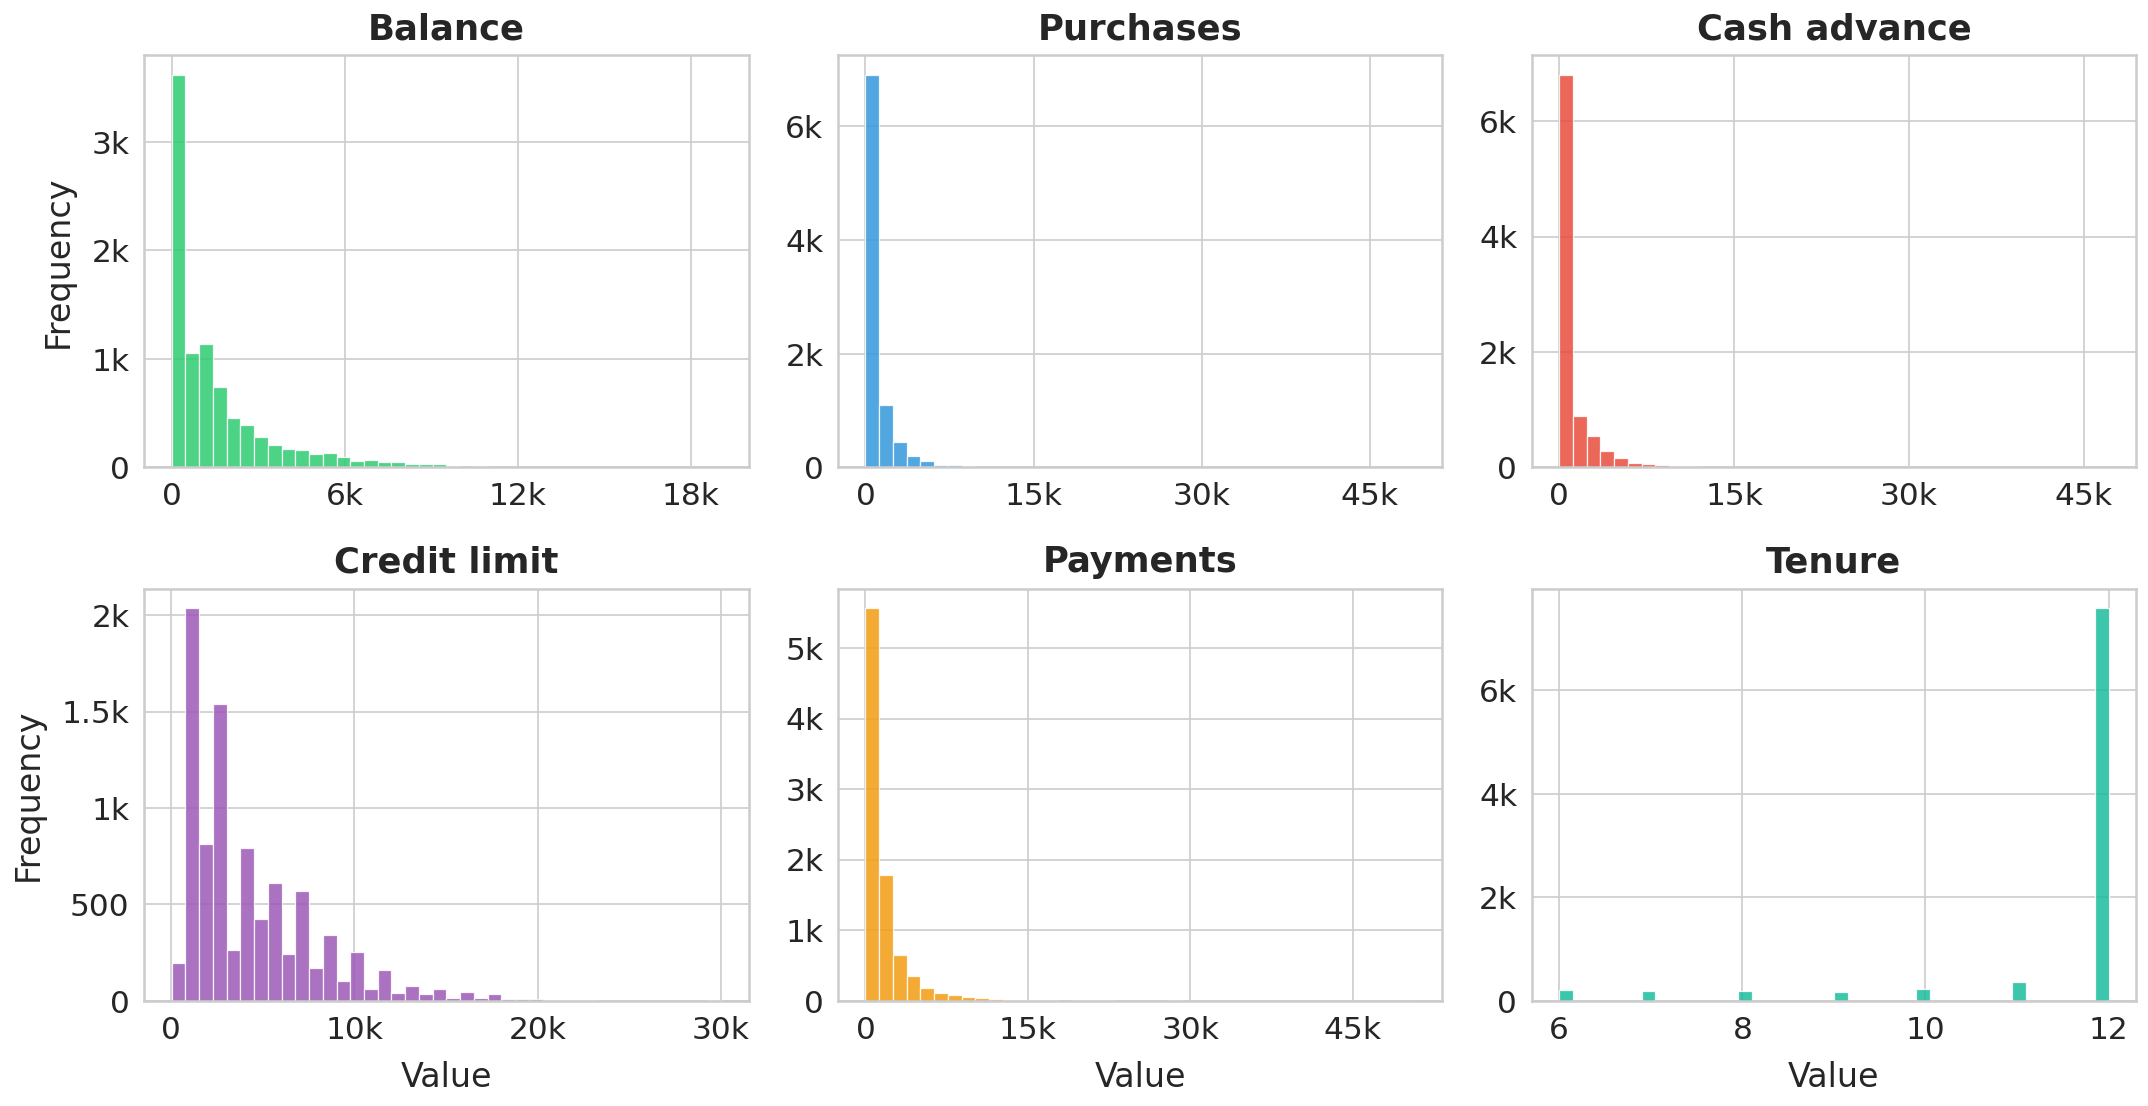
\includegraphics[width=\textwidth]{01_eda_cc_general.png}
    \caption{Distribution of key behavioral features in the CC GENERAL dataset (raw values), showing the right-skewed patterns typical of credit card usage data.}
    \label{fig:eda}
\end{figure*}

\begin{figure*}[!t]
    \centering
    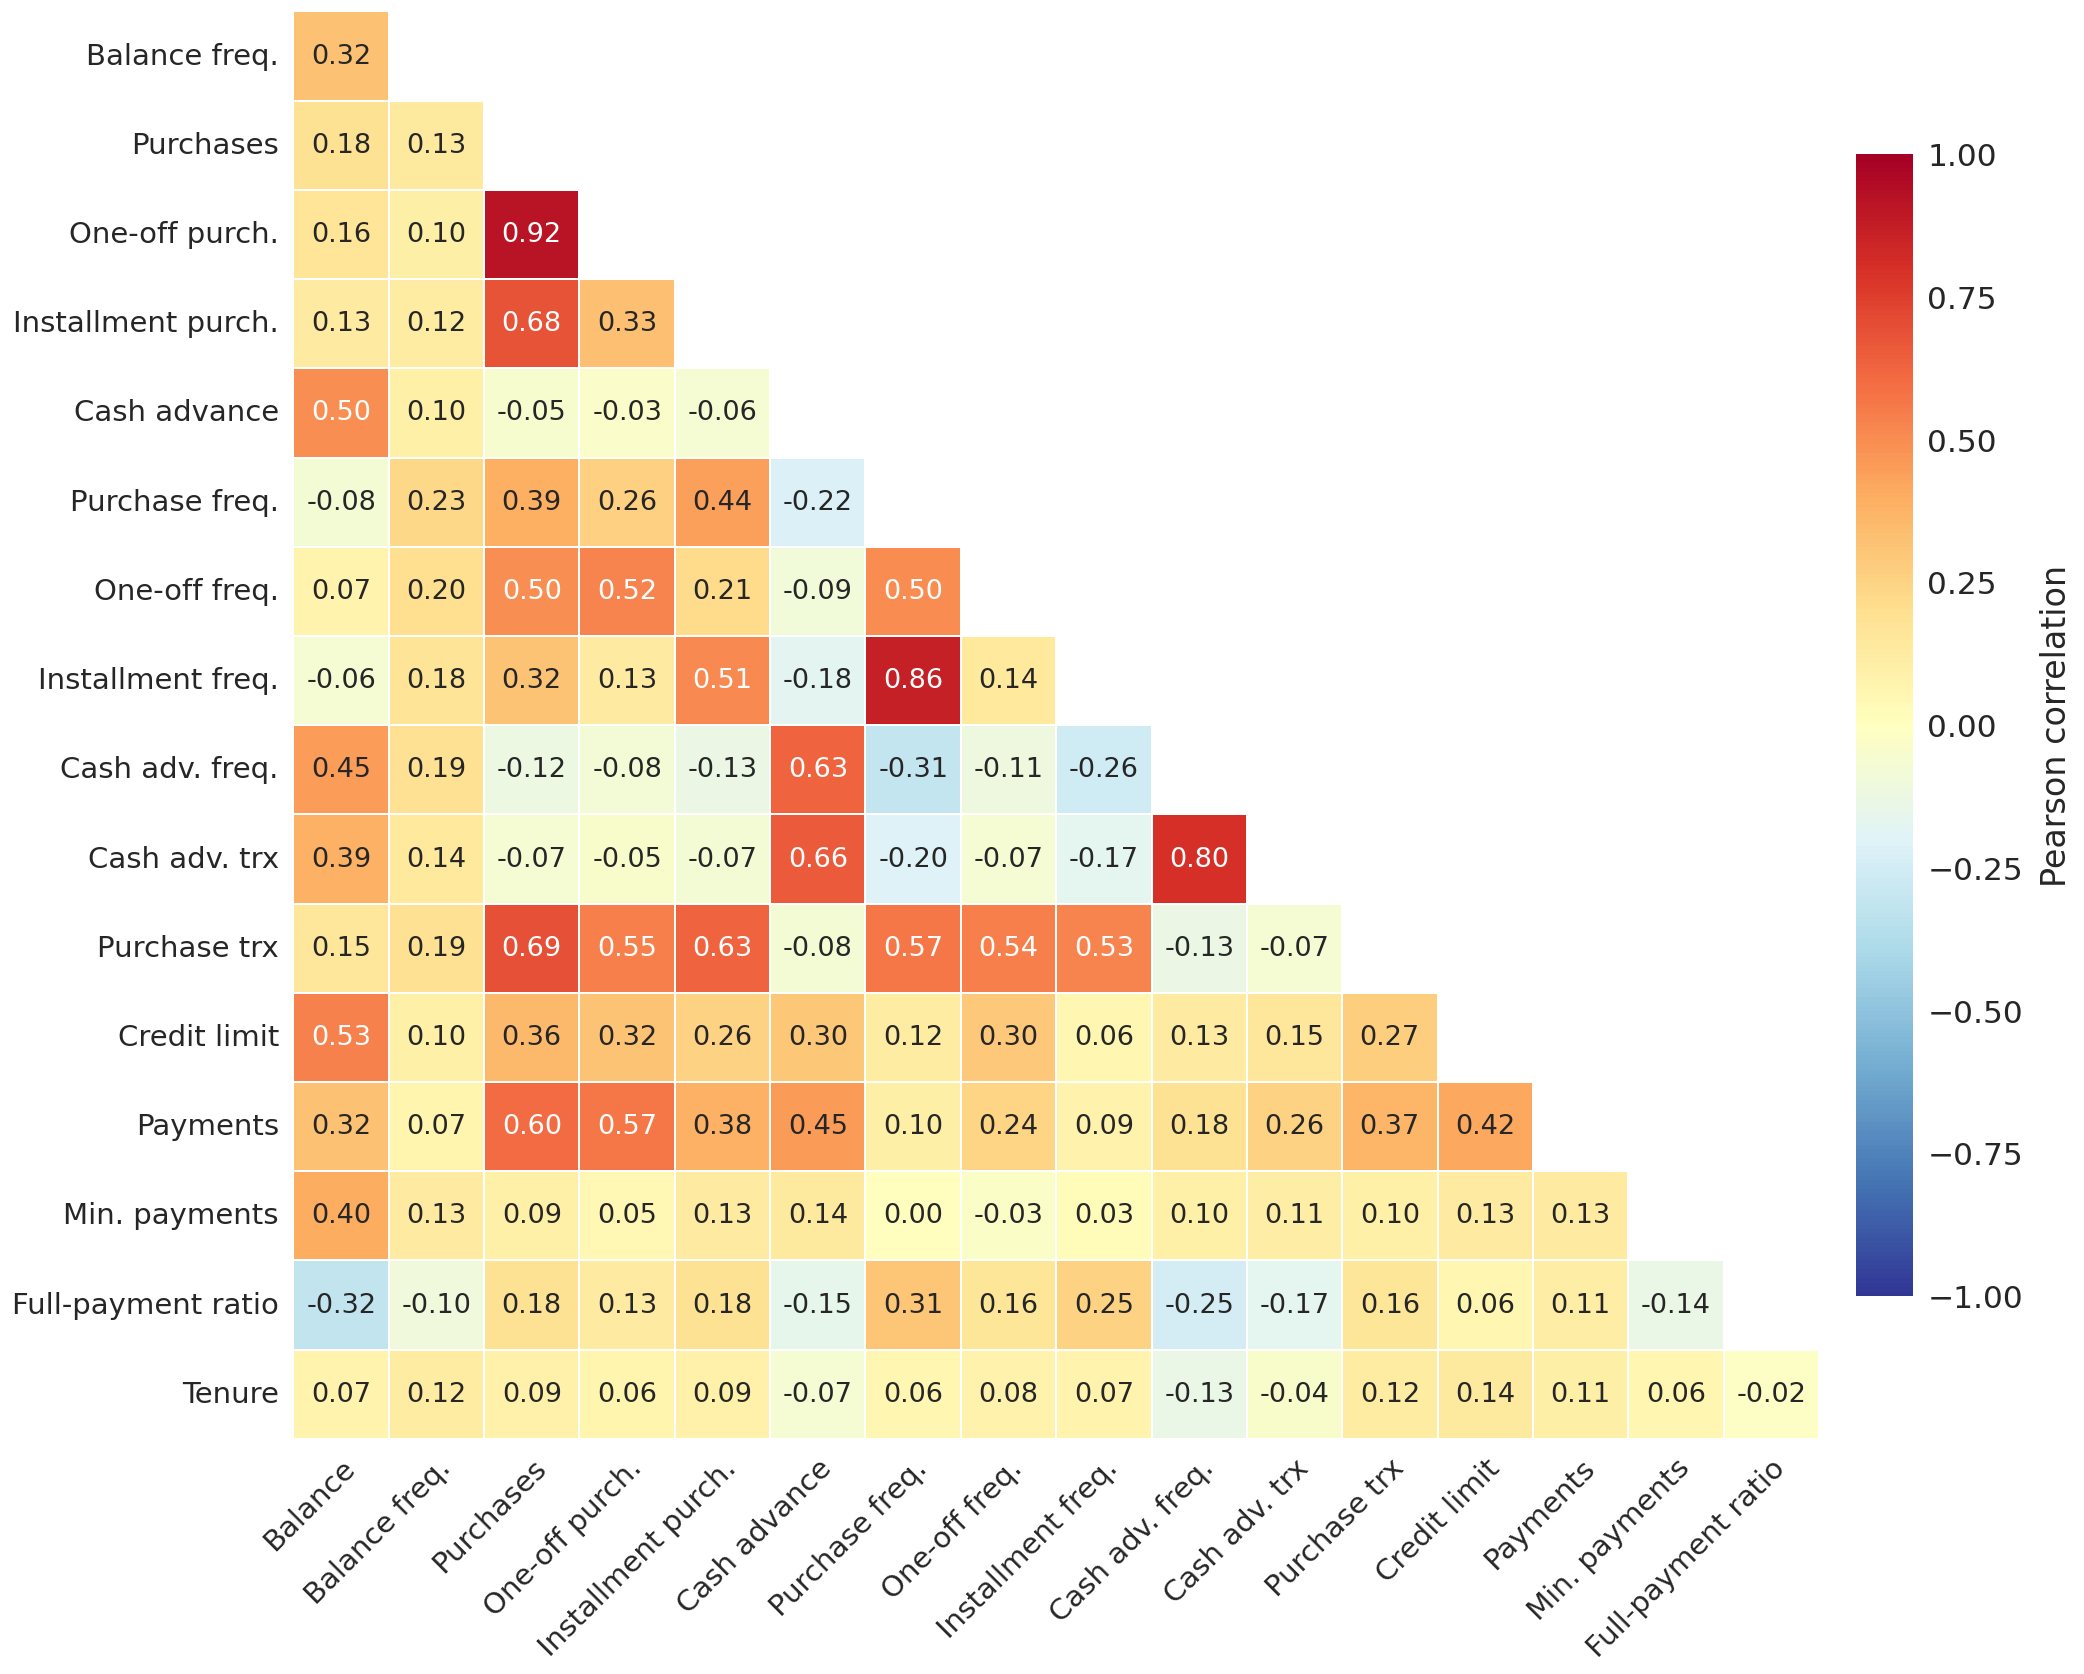
\includegraphics[width=\textwidth]{02_correlation_heatmap.png}
    \caption{Correlation heatmap of the CC GENERAL dataset (lower triangle, Pearson coefficients) revealing multicollinearity among purchase and cash advance features.}
    \label{fig:correlation}
\end{figure*}

\subsubsection{Dataset 2: Fraud Detection}
The 20,000 transactions used from the fraud dataset contain 85 fraudulent cases (0.425\%), a rate higher than that of the complete dataset (0.172\%) but still extreme. After the stratified 80/20 split, the training set contained 16,000 samples (15,932 legitimate and 68 fraudulent) and the test set contained 4,000 samples (3,983 legitimate and 17 fraudulent). The \texttt{scale\_pos\_weight} of XGBoost was therefore computed as $15{,}932/68\approx 234.3$. Because the test set contains only 17 fraudulent transactions, each missed or detected fraud changes recall by 5.9 percentage points, a fact that is considered in the interpretation of all fraud results below.

\subsection{Customer Segmentation Results and Discussion}

Table~\ref{tab:seg_results} summarizes the performance of all four clustering algorithms. The results reveal distinct strengths for each approach, and no algorithm dominates on all three indices.

\begin{table}[!t]
\centering
\caption{Customer Segmentation: Algorithm Comparison}
\label{tab:seg_results}
\renewcommand{\arraystretch}{1.3}
\begin{tabular}{|l|c|c|c|c|}
\hline
\textbf{Algorithm} & \textbf{k} & \textbf{SS}$\uparrow$ & \textbf{DBI}$\downarrow$ & \textbf{CHI}$\uparrow$ \\
\hline
K-Means & 3 & 0.2376 & 1.4564 & \textbf{2846.26} \\
Hierarchical & 3 & 0.1808 & 1.6443 & 2050.65 \\
DBSCAN$^{\dagger}$ & 2 & \textbf{0.3707} & \textbf{0.7163} & 120.75 \\
GMM & 10 & 0.0053 & 2.5924 & 703.05 \\
\hline
\end{tabular}
\\[4pt]
\footnotesize{SS = Silhouette Score, DBI = Davies-Bouldin Index, CHI = Calinski-Harabasz Index. $\uparrow$ = higher is better, $\downarrow$ = lower is better. Bold indicates best per metric. $^{\dagger}$Indices for DBSCAN are computed on the 8,223 non-noise customers only; 727 customers (8.1\%) are labeled as noise.}
\end{table}

\subsubsection{K-Means}

K-Means achieved the highest Calinski-Harabasz Index (2846.26), the second-best Silhouette Score (0.2376), and the second-best Davies-Bouldin Index (1.4564), with an optimal $k=3$. The Silhouette Score peaks at $k=3$ (0.2376), compared with 0.2332 at $k=2$ and 0.2102 at $k=4$, and does not recover for larger $k$, remaining between 0.199 and 0.208 up to $k=10$. The inertia curve (Fig.~\ref{fig:kmeans}) decreases smoothly from 109,508 at $k=2$ to 87,517 at $k=3$ and 76,739 at $k=4$, without a sharp elbow, so that the Elbow criterion alone would be ambiguous and the Silhouette maximum is the decisive criterion, a situation that is common when the Elbow method is used on behavioral banking data \cite{syakur2018integration,raiter2021}. The three clusters contain 2,043 (22.8\%), 4,608 (51.5\%), and 2,299 (25.7\%) customers.

\begin{figure*}[!t]
    \centering
    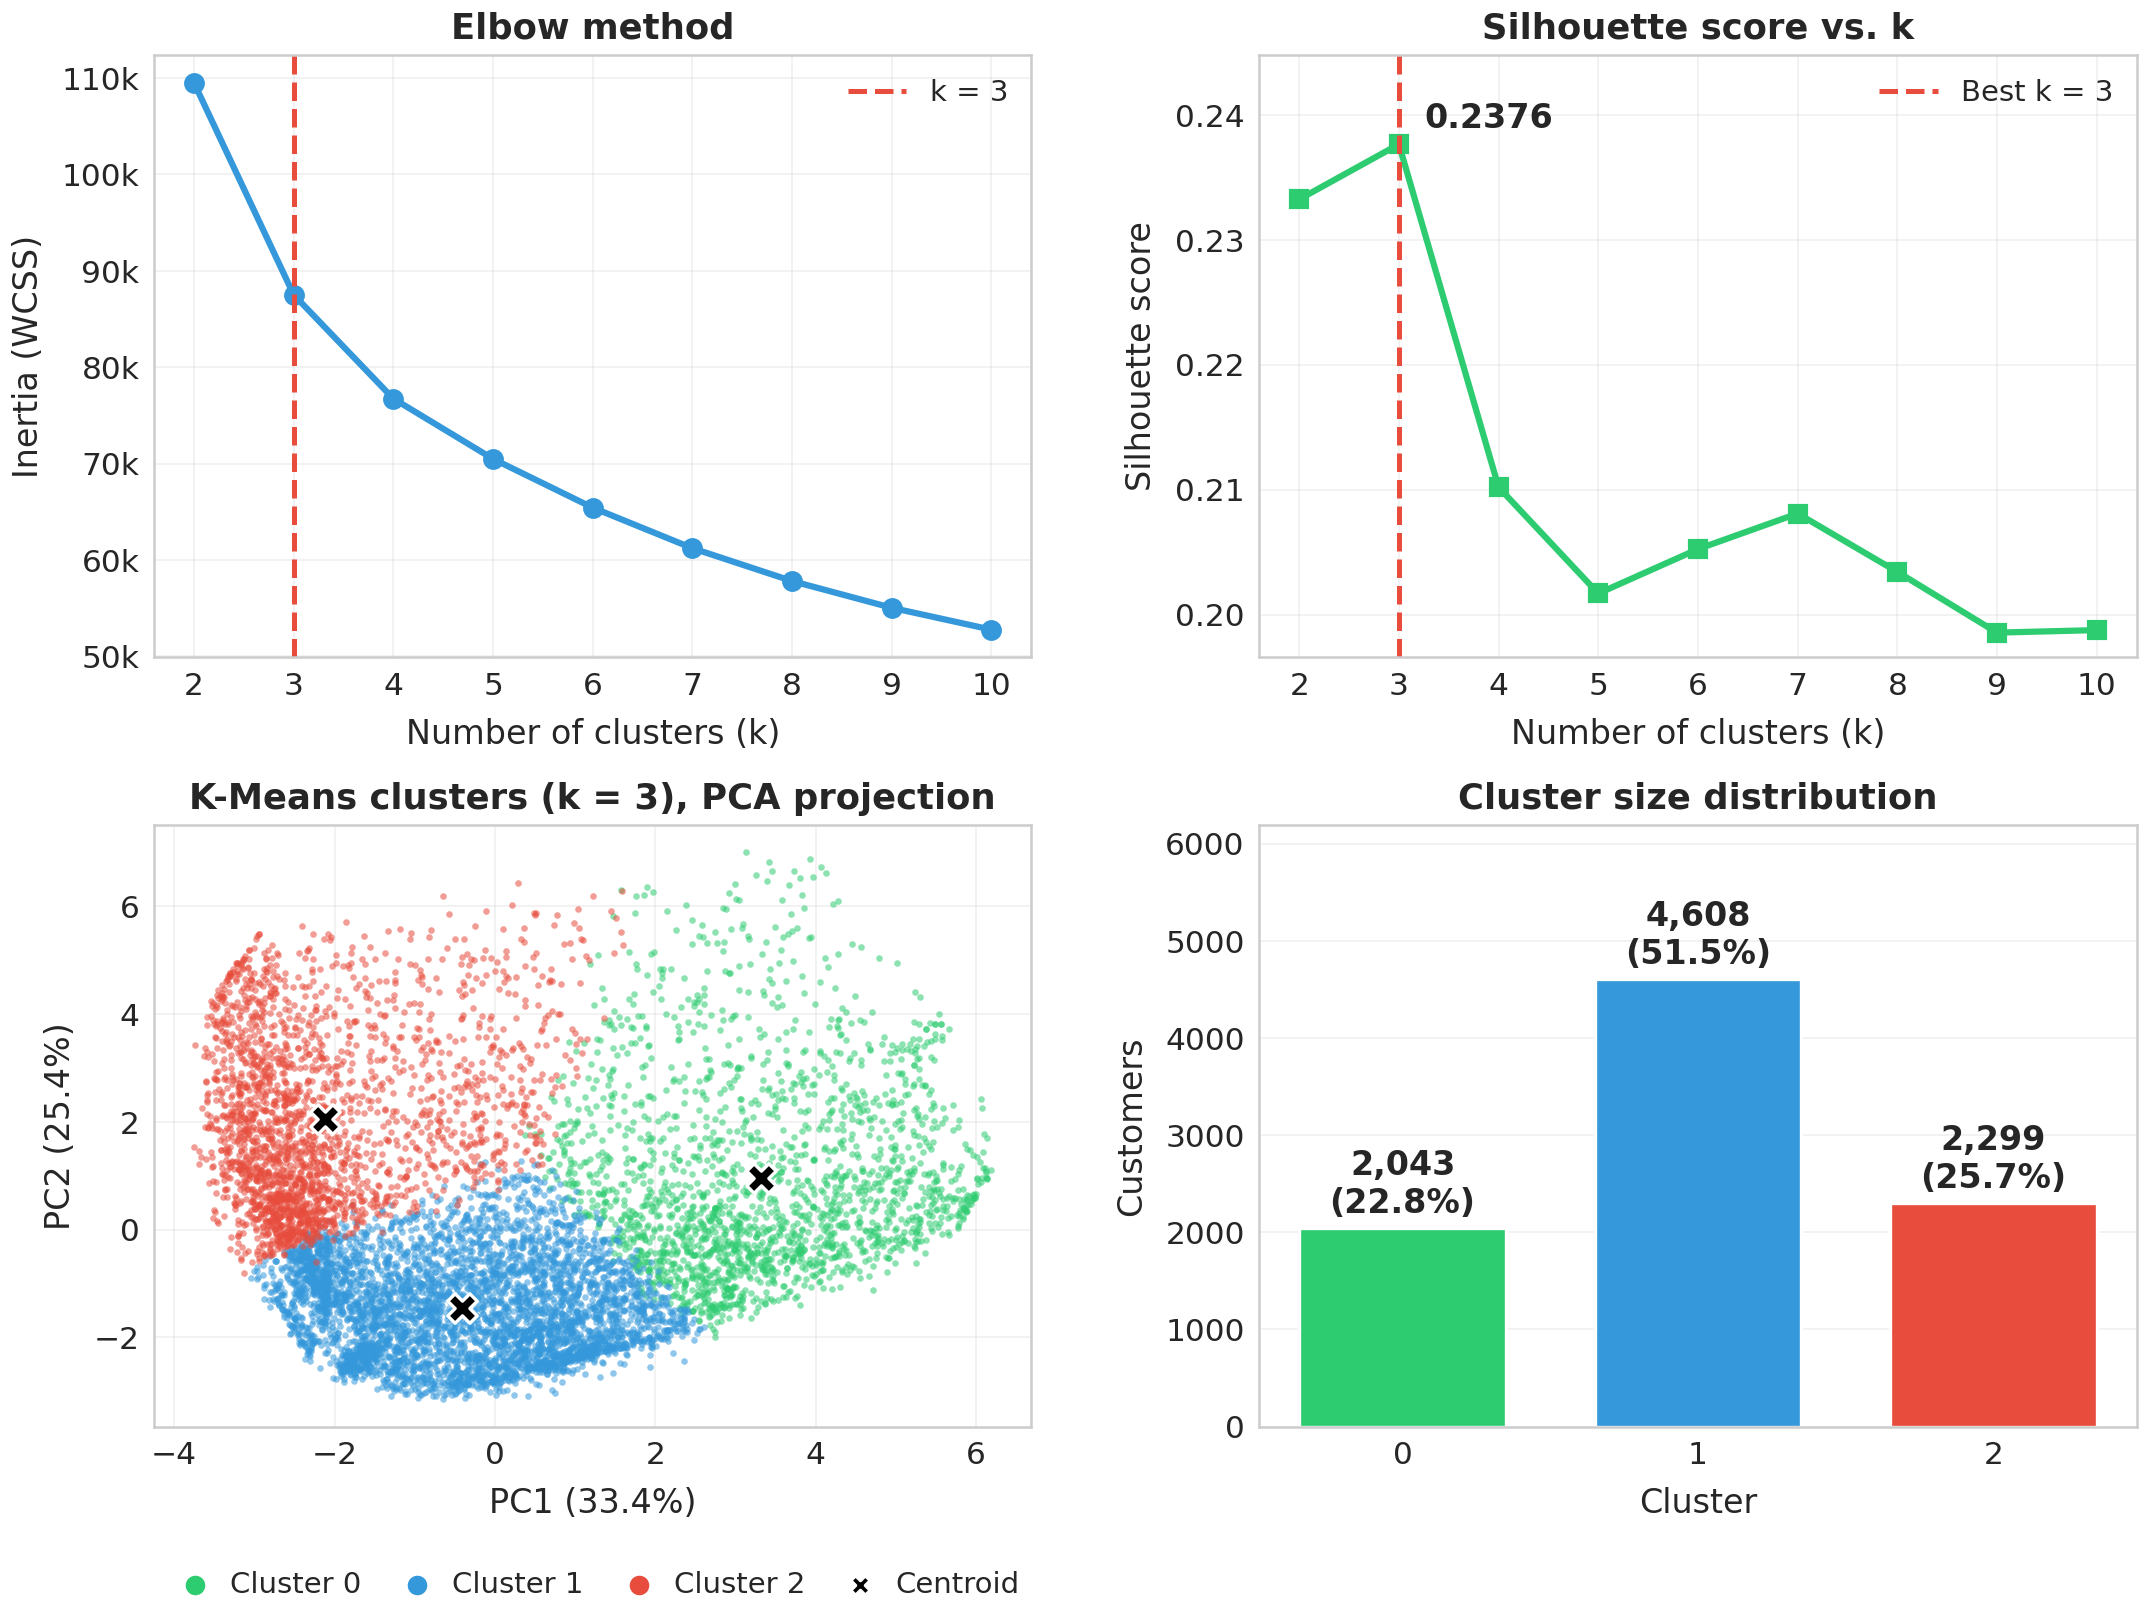
\includegraphics[width=\textwidth]{03_kmeans_analysis.png}
    \caption{K-Means clustering analysis. Top left: Elbow curve of inertia; top right: Silhouette score for $k=2$ to $10$ with the maximum at $k=3$; bottom left: PCA projection of the clusters with centroids; bottom right: cluster sizes with percentages.}
    \label{fig:kmeans}
\end{figure*}

The mean raw feature values of the three clusters (Table~\ref{tab:profiles}) allow the segments to be interpreted as behavioral personas. Cluster~0 (22.8\%) consists of high-value active spenders, who make by far the largest purchases (mean 3,234, of which about 1,235 are installment purchases), show a purchase frequency of 0.91, hold the highest credit limits (6,623), and make the largest payments (3,318). Cluster~1 (51.5\%) is the large group of moderate, low-engagement users, with low balances (564), small purchases (392), a purchase frequency of 0.46, and the smallest credit limits (3,069). Cluster~2 (25.7\%) represents cash-advance-reliant revolvers, whose mean cash advance (2,940) and balance (3,212) are the highest of all groups, whose purchase frequency is only 0.19, and who almost never pay their balance in full (full-payment ratio of 0.03). From a business perspective, the three personas suggest differentiated actions in the manner reported in earlier banking segmentation studies \cite{fouladifar2016,gopalakrishnan2024}: rewards, premium products, and credit limit reviews for the first group, activation and cross-selling campaigns for the second group, and repayment support and early-warning monitoring for the third group, whose reliance on cash advances and low repayment is typically associated with higher credit risk.

\begin{table}[!t]
\centering
\caption{K-Means Cluster Profiles (Mean Raw Feature Values)}
\label{tab:profiles}
\renewcommand{\arraystretch}{1.2}
\begin{tabular}{|l|r|r|r|r|}
\hline
\textbf{Feature} & \textbf{C0} & \textbf{C1} & \textbf{C2} & \textbf{All} \\
\hline
Customers & 2,043 & 4,608 & 2,299 & 8,950 \\
\hline
Balance & 1,967 & 564 & 3,212 & 1,564 \\
\hline
Purchases & 3,234 & 392 & 247 & 1,003 \\
\hline
Cash advance & 582 & 176 & 2,940 & 979 \\
\hline
Purchase freq. & 0.91 & 0.46 & 0.19 & 0.49 \\
\hline
Cash adv. freq. & 0.08 & 0.04 & 0.37 & 0.14 \\
\hline
Credit limit & 6,623 & 3,069 & 5,460 & 4,494 \\
\hline
Payments & 3,318 & 735 & 2,325 & 1,733 \\
\hline
Full-payment ratio & 0.24 & 0.18 & 0.03 & 0.15 \\
\hline
\end{tabular}
\end{table}

The absolute Silhouette Score of 0.2376 is below the level that is conventionally read as indicating well-separated groups, and the PCA projection shows that the three clusters form adjacent regions of one continuous cloud instead of isolated islands. The segmentation therefore partitions a behavioral continuum into practically useful regions and does not reveal naturally disconnected customer types, which is the realistic expectation for credit card behavior and is consistent with the moderate validity values reported for bank customer data in the literature \cite{aryuni2018,barkhordar2021}.

\subsubsection{Hierarchical Clustering}

Agglomerative clustering with Ward's linkage produced a Silhouette Score of 0.1808, a Davies-Bouldin Index of 1.6443, and a Calinski-Harabasz Index of 2050.65 for $k=3$. The dendrogram (Fig.~\ref{fig:hierarchical}) shows that the cut at three clusters lies well above the many small merges at low heights, which supports the choice of a small number of segments. The resulting clusters (3,528, 3,838, and 1,584 customers) are more balanced in size than those of K-Means, but they are less compact, so that all three indices are worse than for K-Means. The two partitions are nevertheless qualitatively similar, in agreement with the observation that hierarchical clustering yields groups comparable to K-Means on bank customers \cite{aliyev2020}, because Ward's criterion and the K-Means objective both minimize within-cluster variance. The greedy and irreversible merge decisions of the hierarchical procedure explain its slightly inferior quality, whereas its principal advantage is the dendrogram, which allows analysts to inspect the segmentation at several granularities, a useful property for exploratory CRM analysis \cite{kikoria2020}. The quadratic cost of the method, in contrast, becomes a practical barrier for customer bases larger than the one analyzed here \cite{hassan2018}.

\begin{figure*}[!t]
    \centering
    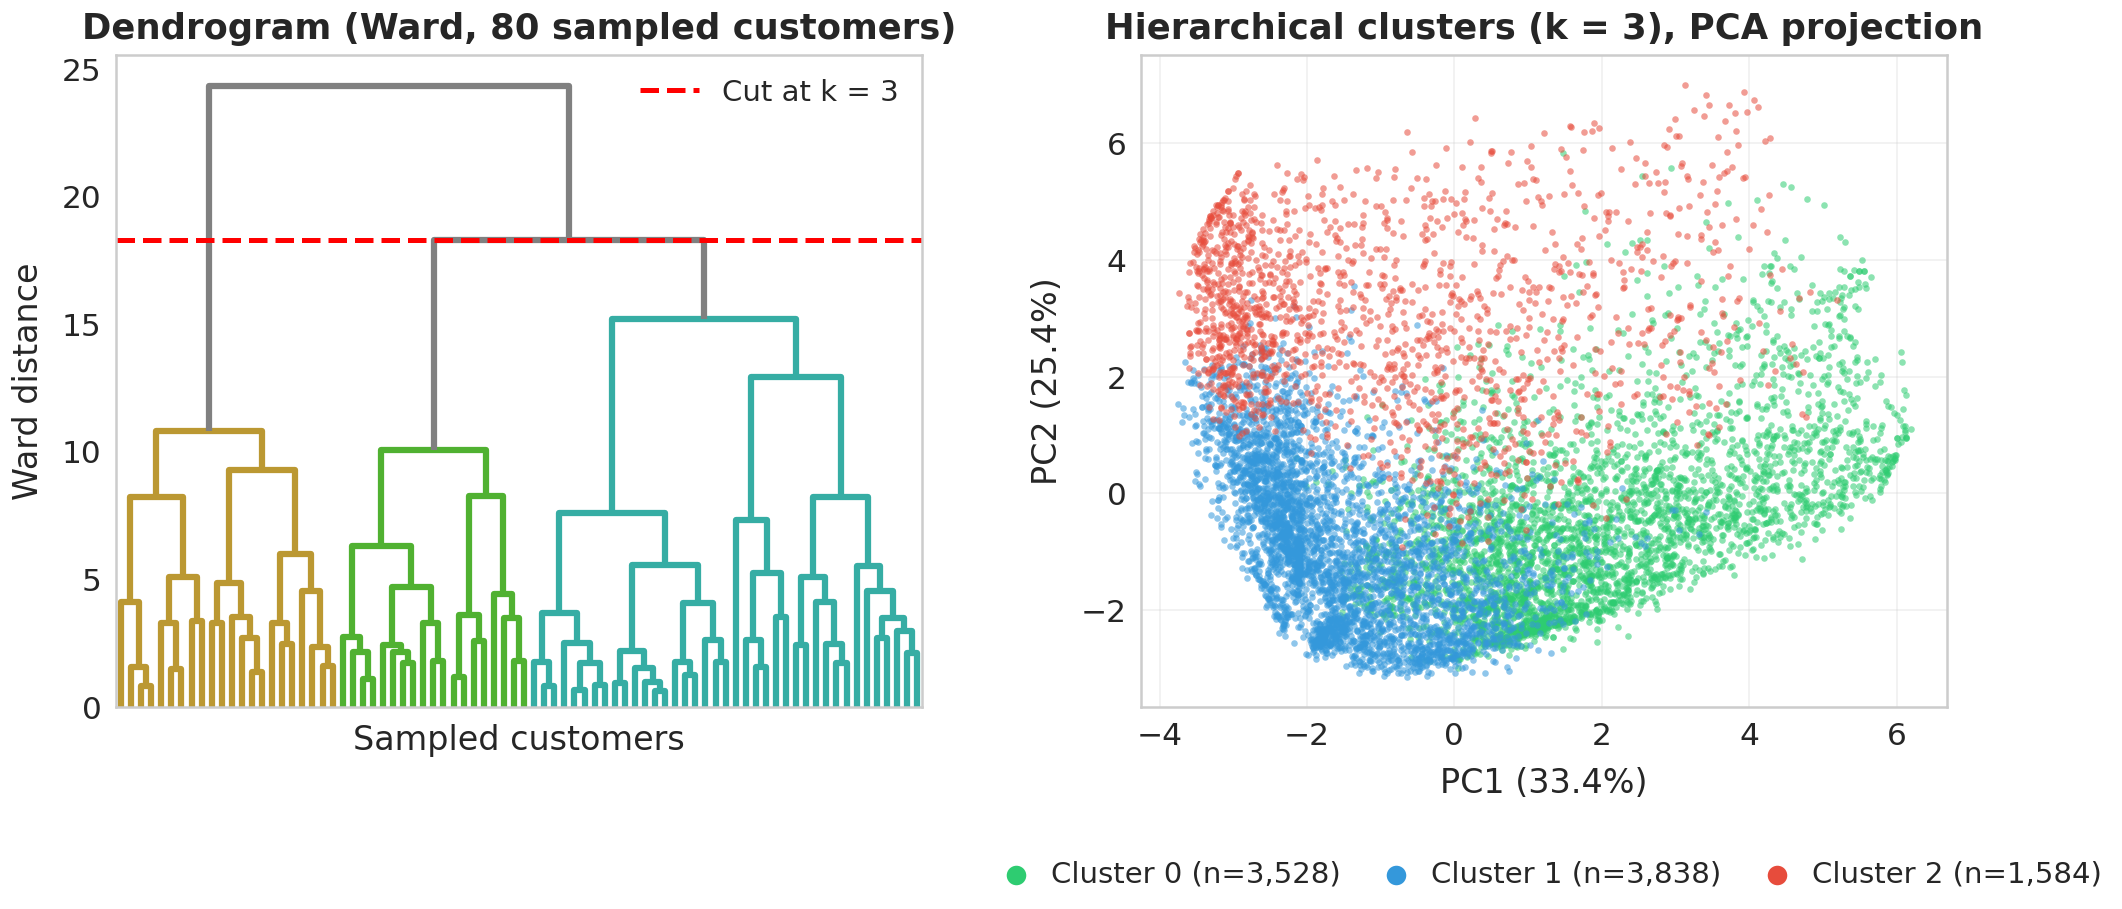
\includegraphics[width=\textwidth]{04_hierarchical_analysis.png}
    \caption{Hierarchical clustering. Left: dendrogram with Ward linkage for 80 sampled customers and the cut for $k=3$; right: PCA projection of the resulting clusters on all customers.}
    \label{fig:hierarchical}
\end{figure*}

\subsubsection{DBSCAN}

DBSCAN attained the highest Silhouette Score (0.3707) and the lowest Davies-Bouldin Index (0.7163) with the selected parameters $\varepsilon=2.0$ and $MinPts=15$. These values must be interpreted with care. The algorithm identified only two clusters, one containing 8,191 customers and a second containing 32 customers, and it labeled 727 customers (8.1\%) as noise (Fig.~\ref{fig:dbscan}). The first cluster therefore comprises 99.6\% of the non-noise customers, so that the result is essentially one dense core with a small, remote satellite group, and the indices are computed after the 727 noise customers have been removed. When the noise customers are retained as a separate group, the Silhouette Score of the same partition falls to 0.1717, which is lower than that of K-Means. The very low Calinski-Harabasz Index (120.75) points in the same direction, because it rewards partitions with large between-cluster dispersion, which a single dominant cluster cannot provide. In addition, the selected $\varepsilon=2.0$ lies on the upper boundary of the search grid, which indicates that smaller radii fragmented the data into many small groups or excessive noise in the 17-dimensional space, where distances between points become less discriminative. These observations reproduce the parameter selection and density-uniformity difficulties that motivated hybrid K-Means/DBSCAN designs for bank customers \cite{yan2025}. The practical value of DBSCAN in this setting is not the partition but the noise label, since the 727 flagged customers are unusual in their behavior and constitute a natural list for manual review.

\begin{figure*}[!t]
    \centering
    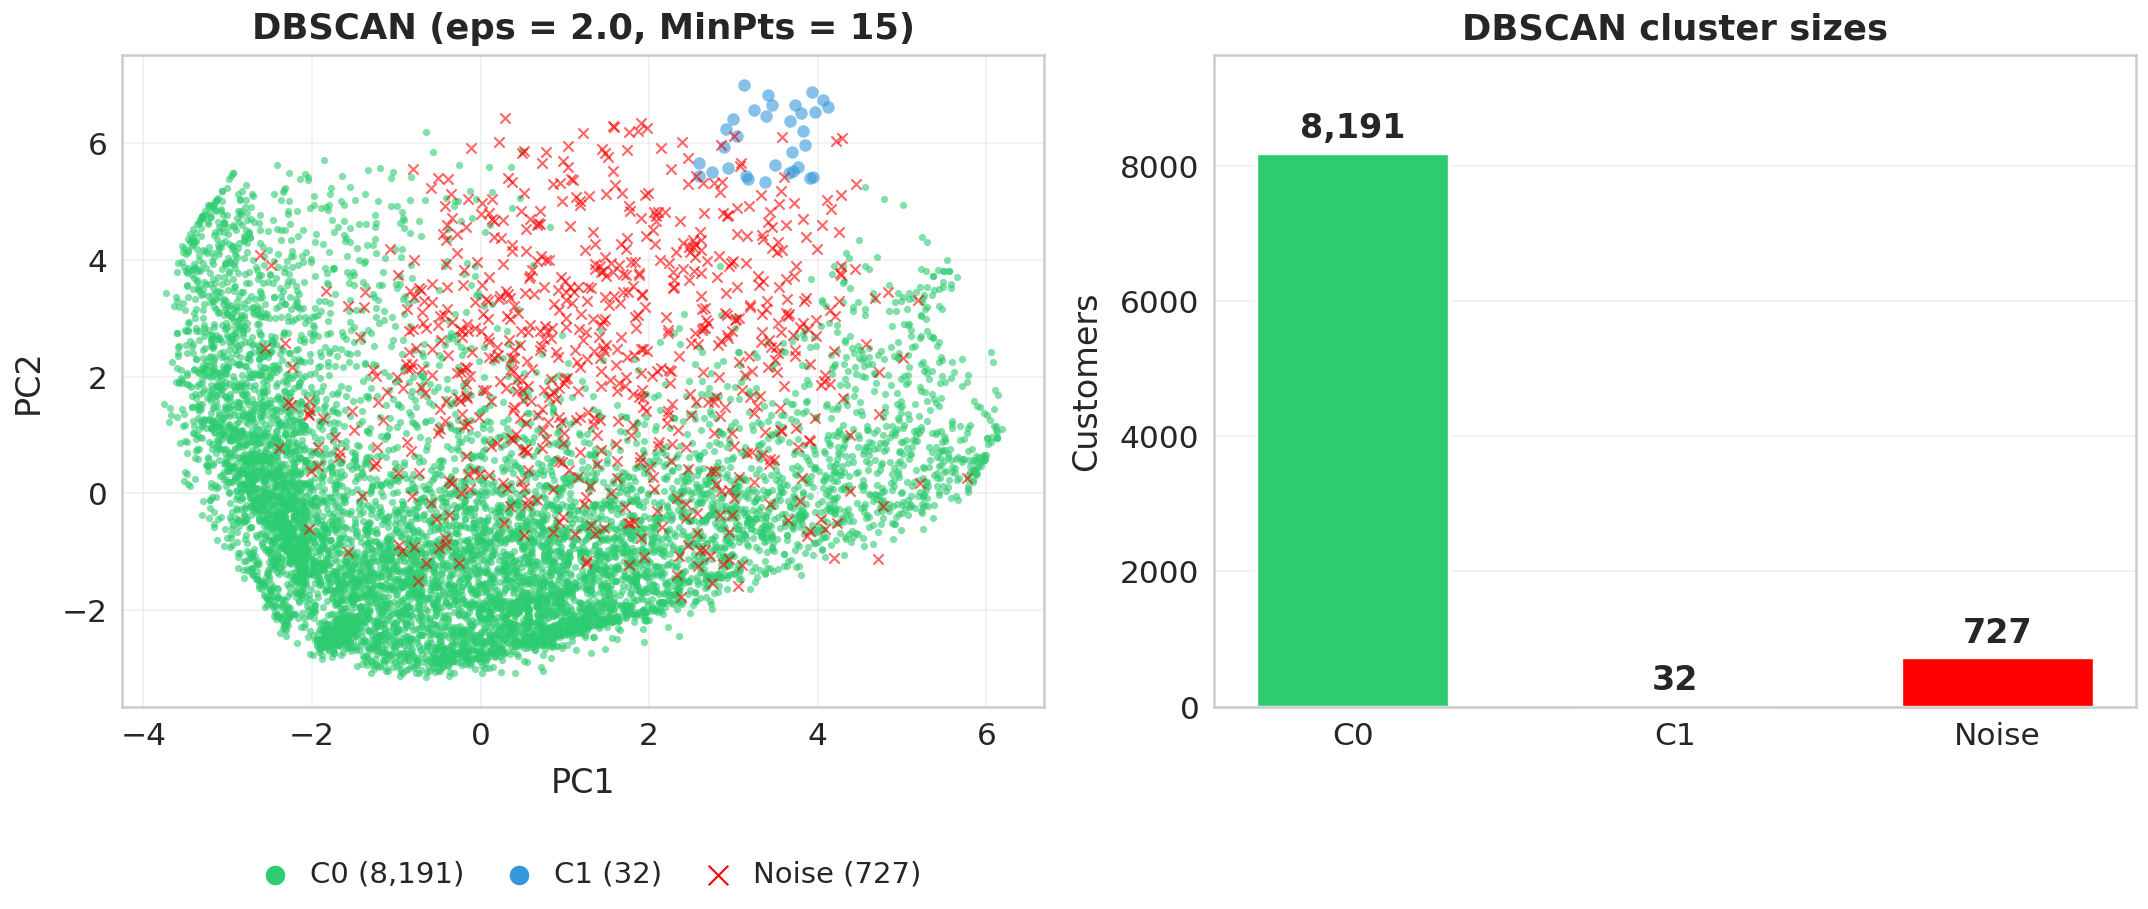
\includegraphics[width=\textwidth]{05_dbscan_analysis.png}
    \caption{DBSCAN clustering. Left: cluster assignments in the PCA plane with noise points marked as red crosses; right: sizes of the two clusters and of the noise group.}
    \label{fig:dbscan}
\end{figure*}

\subsubsection{Gaussian Mixture Model}

The Gaussian mixture model with full covariance selected $n=10$ components through BIC minimization, which is the upper end of the searched range (Fig.~\ref{fig:gmm}). BIC decreased monotonically over the entire range, from 53,144 at two components to $-247{,}944$ at five and $-381{,}171$ at ten components, so that no interior minimum was found and a larger number of components would have been preferred if the search had been extended. The resulting partition yielded the lowest Silhouette Score (0.0053) and the highest Davies-Bouldin Index (2.5924), and its ten clusters range from 342 to 2,016 customers. The continued improvement of BIC together with the near-zero Silhouette Score is explained by the data distribution and not by random noise fitting alone. The behavioral variables are zero-inflated, bounded, and heavy-tailed even after capping, so that a Gaussian mixture needs many overlapping components to approximate the density, and those components overlap strongly in Euclidean space, which the Silhouette Score penalizes. The model is therefore a good density estimator but a poor segmentation device for this dataset. Its soft assignments remain valuable for tasks such as churn scoring, where probabilities and not labels are required \cite{saxena2023}, and the comparison with K-Means for other data types confirms that the benefit of soft membership comes with higher model complexity \cite{patel2020clustering}. The ten-component model has 1,709 free parameters, which is also unattractive for marketing teams that need a small number of explainable segments.

\begin{figure*}[!t]
    \centering
    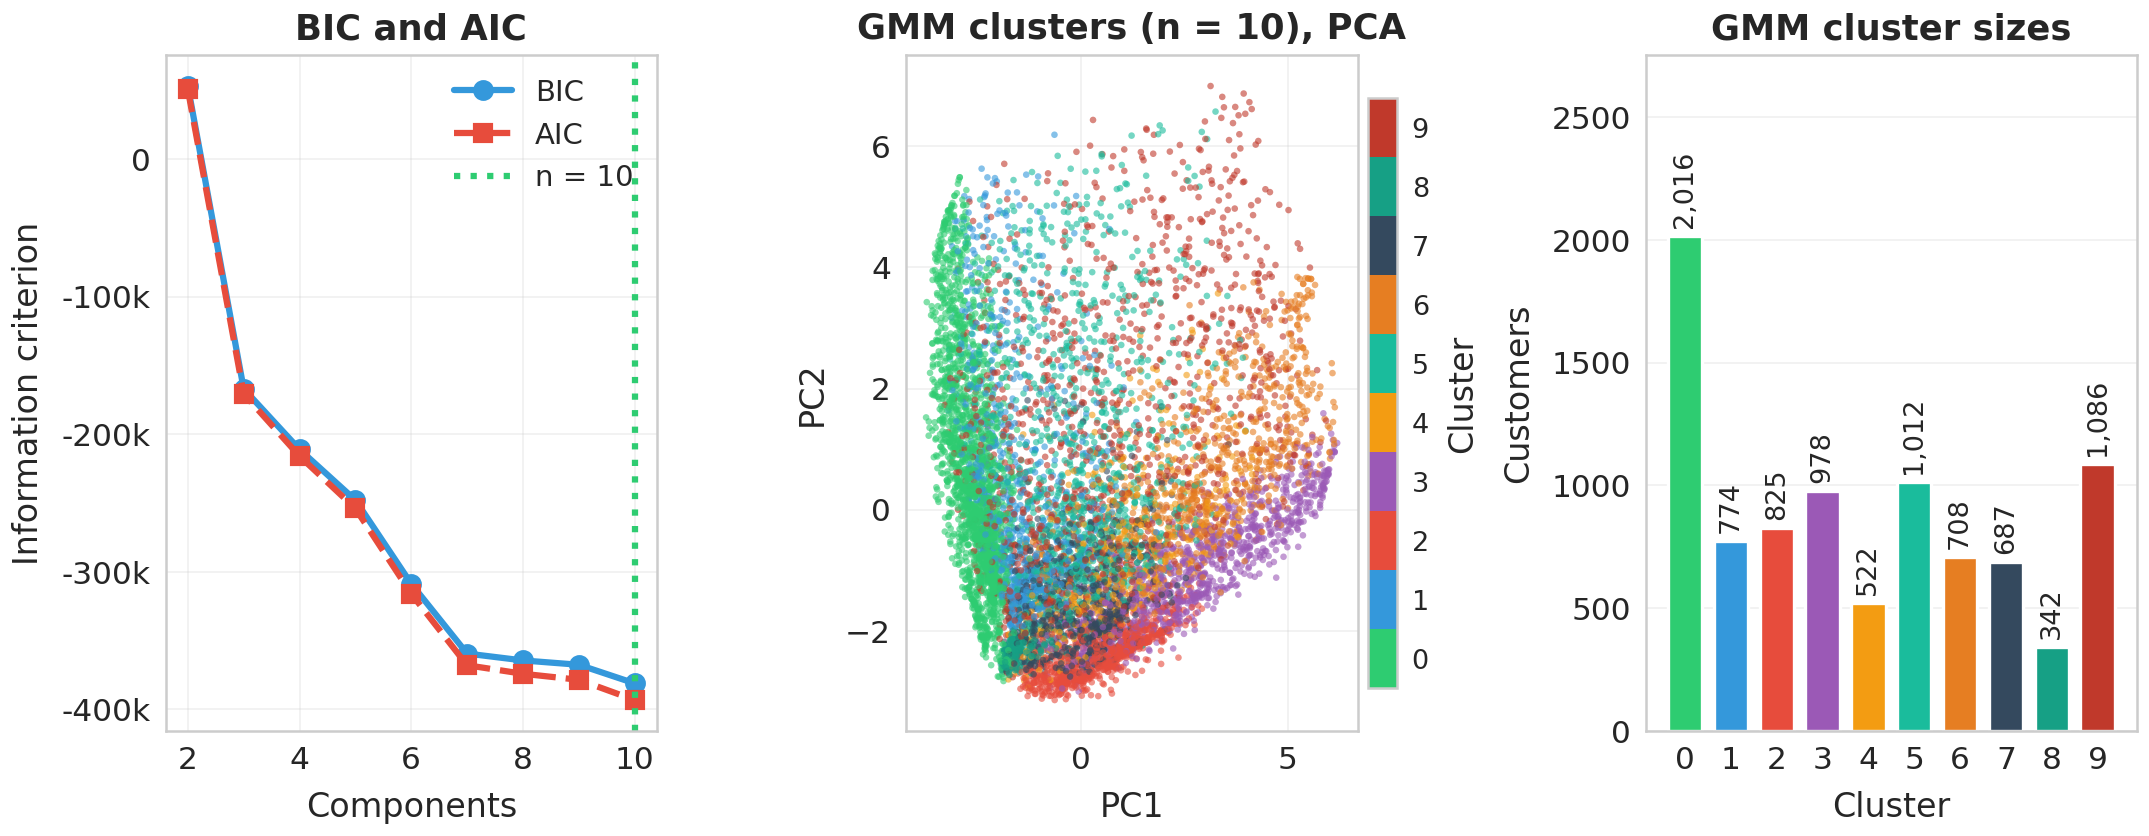
\includegraphics[width=\textwidth]{06_gmm_analysis.png}
    \caption{Gaussian Mixture Model analysis. Left: BIC and AIC against the number of components, both still decreasing at ten components; center: PCA projection of the ten components; right: cluster sizes.}
    \label{fig:gmm}
\end{figure*}

\subsubsection{Segmentation Algorithm Comparison}

Fig.~\ref{fig:seg_comparison} provides a visual comparison across all three metrics. The ranking depends on the metric. DBSCAN leads on the Silhouette Score and Davies-Bouldin Index, but only because the indices are evaluated on a nearly single-cluster, noise-filtered partition. K-Means leads on the Calinski-Harabasz Index, is second on the other two indices, and is the only method that simultaneously delivers more than two interpretable and reasonably balanced clusters. Hierarchical clustering follows K-Means closely, and GMM is clearly the weakest. K-Means is therefore the most suitable algorithm for operational segmentation of this dataset, in line with the prevalence of K-Means in the segmentation literature \cite{gomes2023,das2022}, whereas DBSCAN is better used as a complementary outlier screen.

\begin{figure*}[!t]
    \centering
    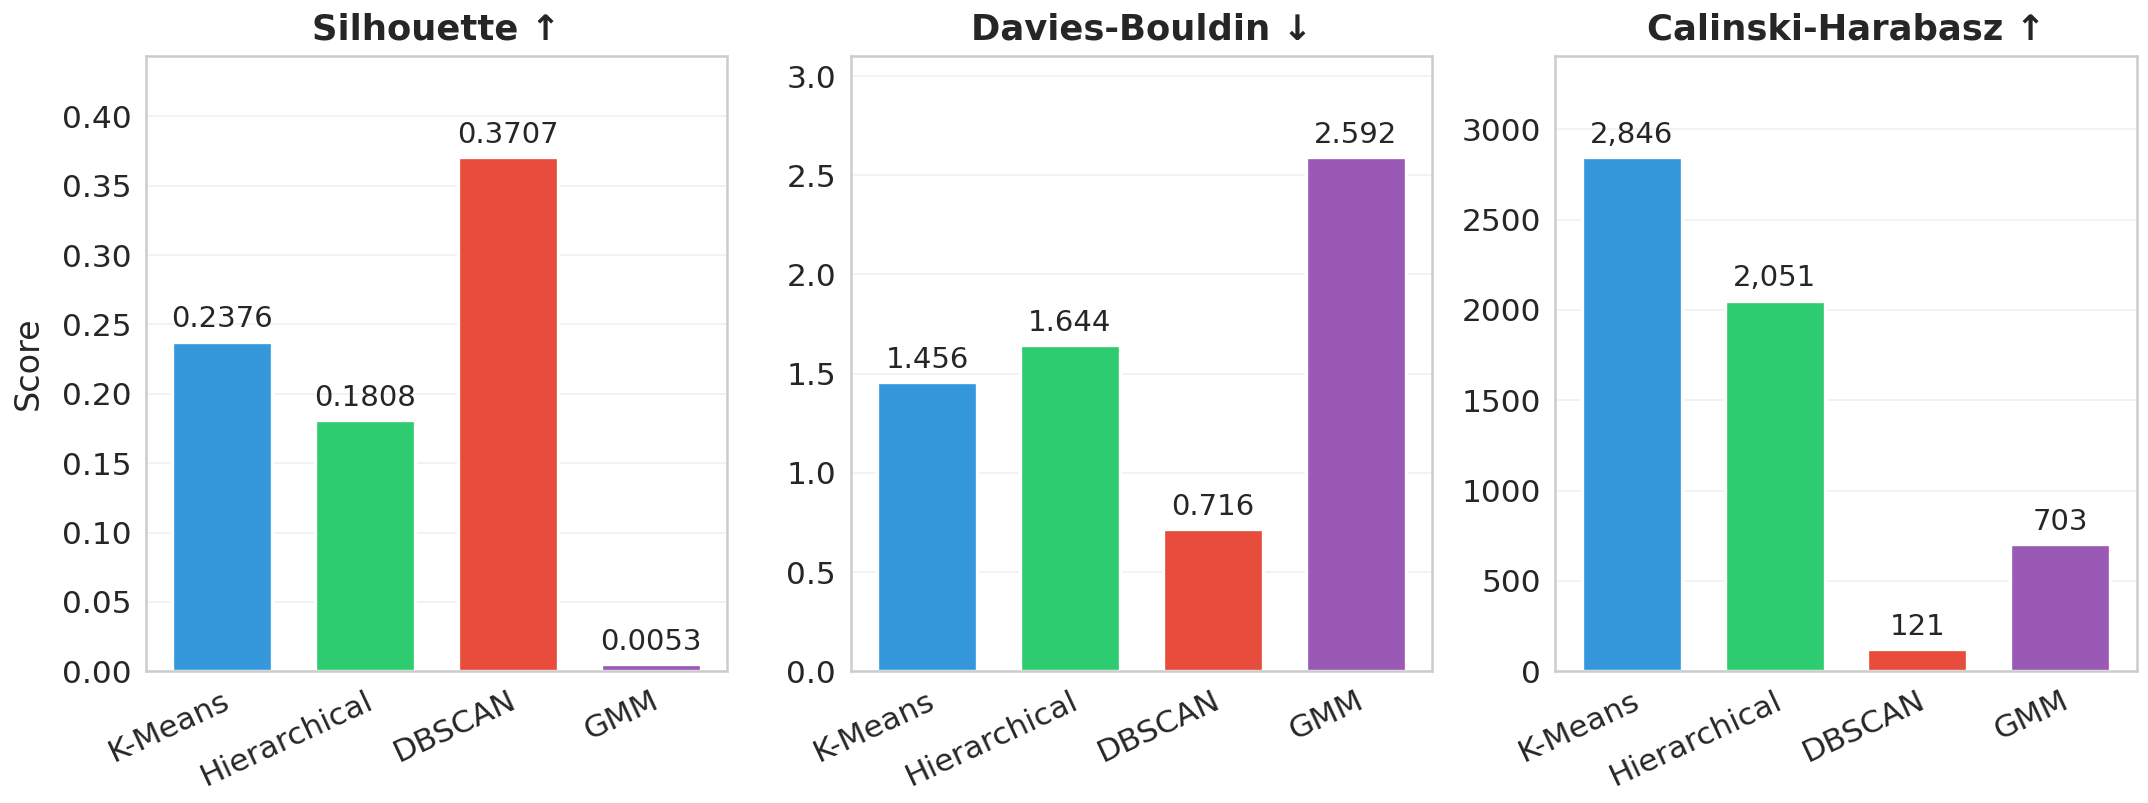
\includegraphics[width=\textwidth]{07_segmentation_comparison.png}
    \caption{Comparison of the four segmentation algorithms by Silhouette Score, Davies-Bouldin Index, and Calinski-Harabasz Index (DBSCAN indices on non-noise customers).}
    \label{fig:seg_comparison}
\end{figure*}

\subsection{Fraud Detection Results and Discussion}

Table~\ref{tab:fraud_results} presents the performance of all four fraud detection algorithms, and Table~\ref{tab:confusion} lists the corresponding confusion matrix counts on the 4,000 test transactions.

\begin{table}[!t]
\centering
\caption{Fraud Detection: Algorithm Performance Comparison}
\label{tab:fraud_results}
\renewcommand{\arraystretch}{1.3}
\begin{tabular}{|l|c|c|c|c|c|c|}
\hline
\textbf{Algorithm} & \textbf{Acc.} & \textbf{Prec.} & \textbf{Rec.} & \textbf{F1} & \textbf{AUC} & \textbf{AP} \\
\hline
Log. Reg. & 0.987 & 0.239 & \textbf{1.000} & 0.386 & 0.998 & 0.570 \\
Rand. For. & 0.999 & 0.882 & 0.882 & 0.882 & 1.000 & 0.961 \\
Isol. For. & 0.994 & 0.333 & 0.353 & 0.343 & 0.987 & 0.428 \\
XGBoost & \textbf{1.000} & \textbf{0.944} & \textbf{1.000} & \textbf{0.971} & \textbf{1.000} & \textbf{1.000} \\
\hline
\end{tabular}
\\[4pt]
\footnotesize{Bold indicates best performance per metric. Acc. = Accuracy, Prec. = Precision, Rec. = Recall, AP = Average Precision. Test set: 4,000 transactions, of which 17 are fraudulent.}
\end{table}

\begin{table}[!t]
\centering
\caption{Confusion Matrix Counts on the Test Set (17 Frauds)}
\label{tab:confusion}
\renewcommand{\arraystretch}{1.2}
\begin{tabular}{|l|r|r|r|r|}
\hline
\textbf{Algorithm} & \textbf{TN} & \textbf{FP} & \textbf{FN} & \textbf{TP} \\
\hline
Log. Reg. & 3,929 & 54 & 0 & 17 \\
\hline
Rand. For. & 3,981 & 2 & 2 & 15 \\
\hline
Isol. For. & 3,971 & 12 & 11 & 6 \\
\hline
XGBoost & 3,982 & 1 & 0 & 17 \\
\hline
\end{tabular}
\end{table}

\subsubsection{Logistic Regression}

Logistic Regression achieved perfect recall (1.000), detecting all 17 fraudulent transactions in the test set, but suffered from poor precision (0.239), generating 54 false positives among 3,983 legitimate transactions (1.4\%). A review queue produced by this model would contain 71 alerts, of which only 17 are genuine, which results in a low F1-Score of 0.386. The ROC-AUC of 0.998 indicates that the model ranks fraudulent transactions almost perfectly above legitimate ones, but the Average Precision of only 0.570 shows that, once the large number of legitimate transactions is taken into account, the ranking is not sharp enough to separate the two classes at the default threshold. The same contrast between a high ROC-AUC and a low precision--recall summary is the phenomenon described for imbalanced data \cite{saito2015precision}. Balanced class weights push the linear decision boundary toward the minority class, which secures recall at the expense of many false alarms. Fig.~\ref{fig:lr_eval} shows the confusion matrix and evaluation curves. A higher decision threshold or probability calibration, as discussed for unbalanced data in \cite{dal2014learned}, would probably improve precision without sacrificing the excellent ranking.

\begin{figure*}[!t]
    \centering
    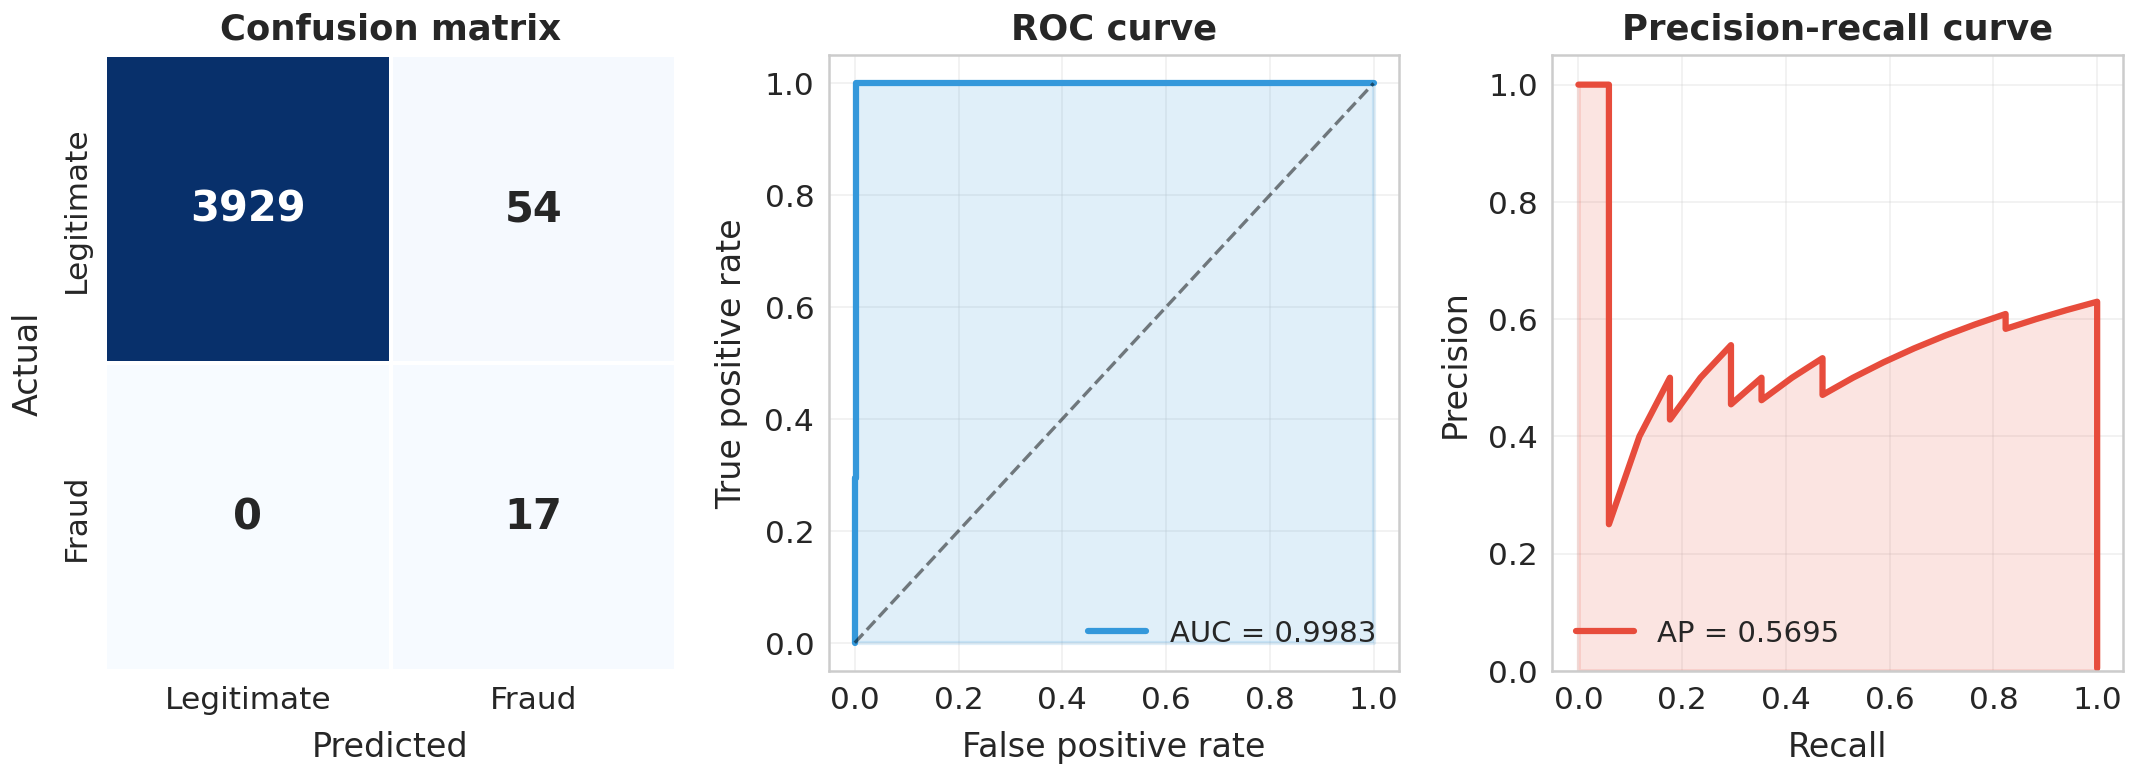
\includegraphics[width=\textwidth]{logistic_regression_eval.png}
    \caption{Logistic Regression evaluation. Left: confusion matrix showing a high false positive count despite perfect recall; center: ROC curve (AUC = 0.998); right: precision--recall curve (AP = 0.570).}
    \label{fig:lr_eval}
\end{figure*}

\subsubsection{Random Forest}

Random Forest delivered strong overall performance, with a precision and recall of 0.882 each (15 of 17 frauds detected, 2 false positives), an F1-Score of 0.882, a ROC-AUC of 0.9998, and an Average Precision of 0.961. The ensemble of 200 depth-limited trees captures non-linear relationships among the anonymized components while keeping the false alarm rate at 0.05\%, which is considerably lower than that of Logistic Regression, in agreement with the earlier finding that random forests outperform logistic regression and support vector machines on real credit card data \cite{bhattacharyya2011data}. The feature importance analysis (Fig.~\ref{fig:rf_importance}) shows that the model relies mainly on a small number of components: V14 (0.186), V4 (0.140), V3 (0.117), V10 (0.100), and V17 (0.081) together account for 62\% of the total importance. Because V1--V28 are anonymized principal components, the importance ranking identifies which components carry fraud-related signal but does not permit a semantic interpretation such as transaction velocity or amount deviation. Fig.~\ref{fig:rf_eval} shows the detailed evaluation of this model.

\begin{figure*}[!t]
    \centering
    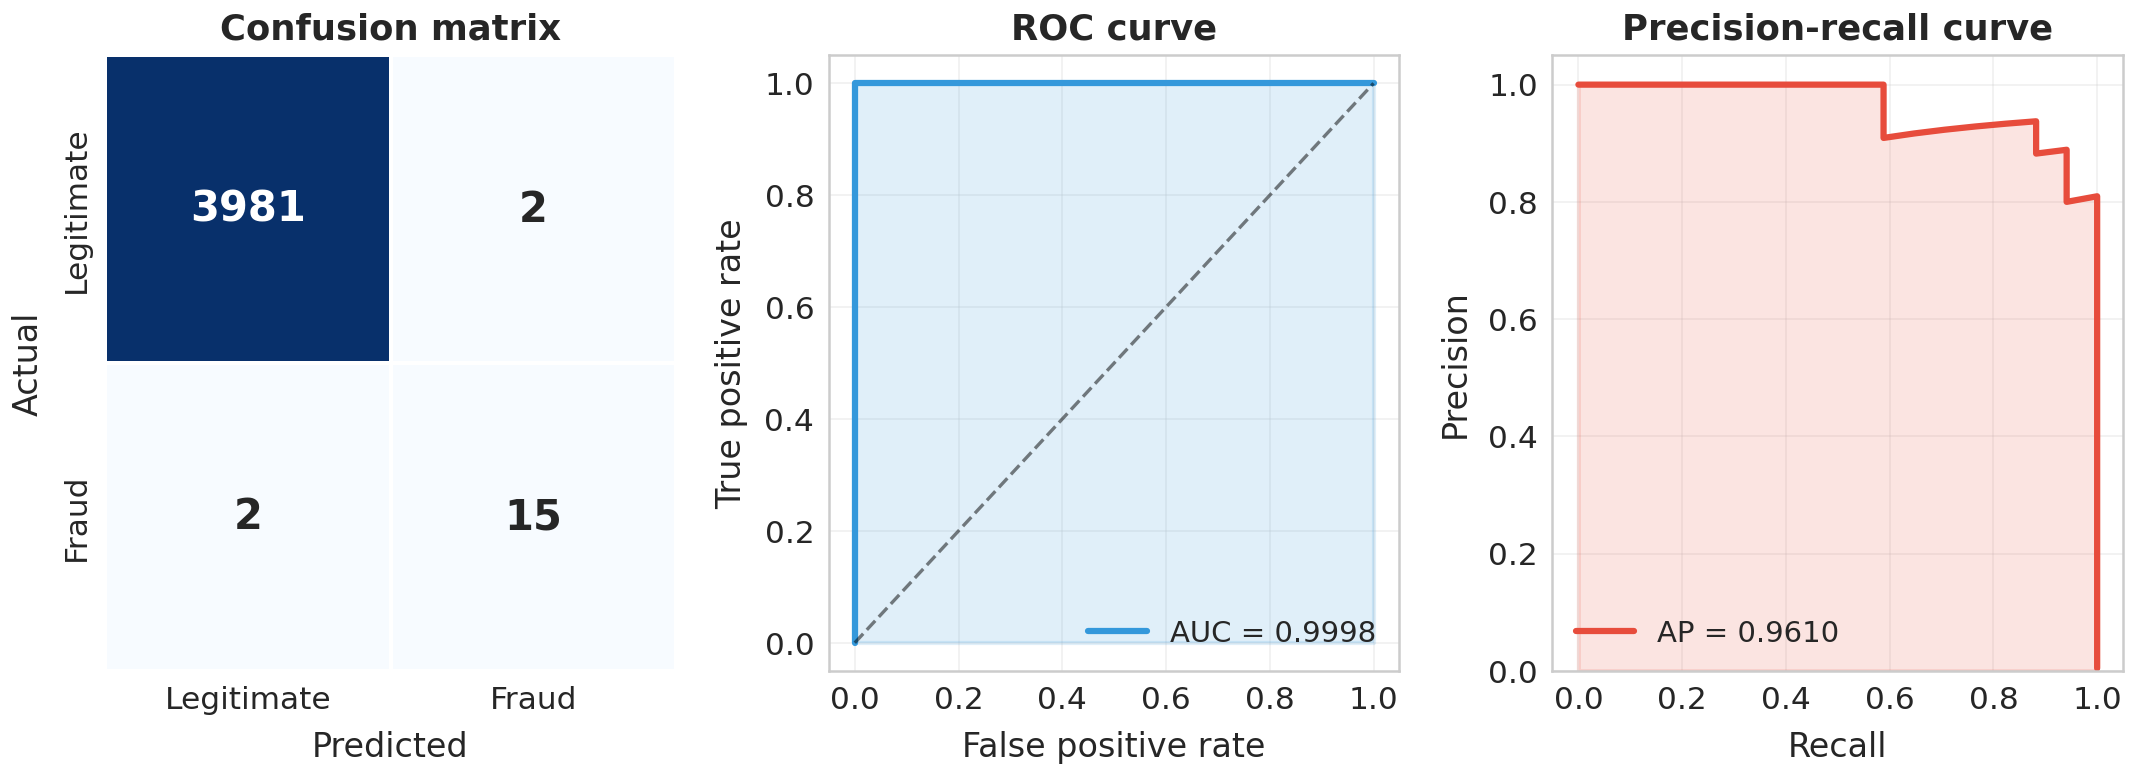
\includegraphics[width=\textwidth]{random_forest_eval.png}
    \caption{Random Forest evaluation. Left: confusion matrix showing a balanced precision--recall trade-off; center: ROC curve (AUC = 1.000); right: precision--recall curve (AP = 0.961).}
    \label{fig:rf_eval}
\end{figure*}

\begin{figure}[!t]
    \centering
    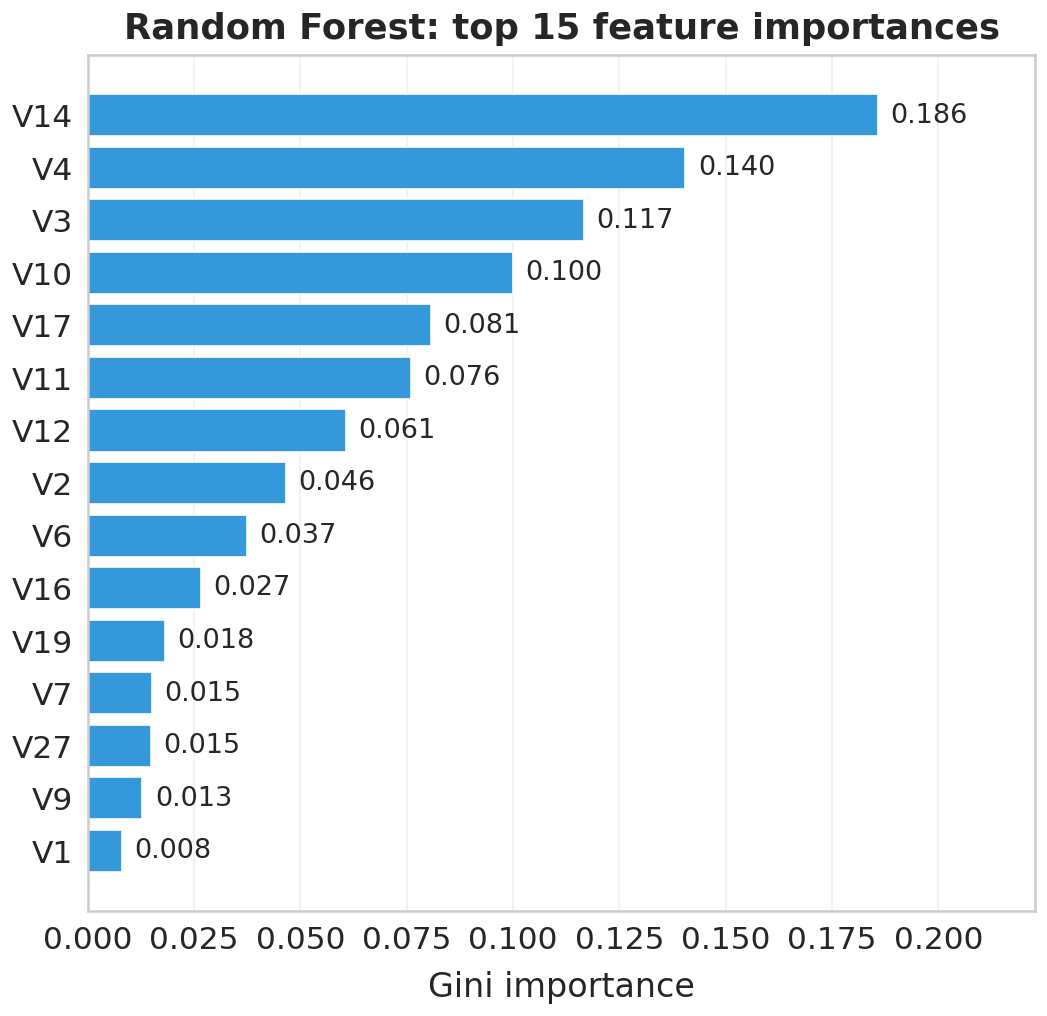
\includegraphics[width=\columnwidth]{rf_feature_importance.png}
    \caption{Random Forest top 15 feature importances, with V14, V4, V3, V10, and V17 as the most influential components for fraud detection.}
    \label{fig:rf_importance}
\end{figure}

\subsubsection{Isolation Forest}

As an unsupervised anomaly detector, Isolation Forest achieved modest classification metrics (F1 = 0.343, Precision = 0.333, Recall = 0.353), with 6 of 17 frauds detected, 12 false positives, and 11 missed frauds. Its ROC-AUC of 0.987 (Fig.~\ref{fig:iso_eval}), however, shows that the anomaly score alone ranks most fraudulent transactions above most legitimate ones, even though the model never used a label during training. The gap between the strong ranking and the weak thresholded decision arises because many fraudulent transactions resemble ordinary ones in the principal component space and are therefore not isolated quickly, and because the contamination-based threshold flags only the most extreme 0.425\% of transactions. The result confirms the usual role of unsupervised detectors: they are valuable when labeled fraud is scarce or when new attack patterns must be surfaced \cite{bolton2002statistical}, but they are outperformed by supervised models when sufficient labels exist.

\begin{figure*}[!t]
    \centering
    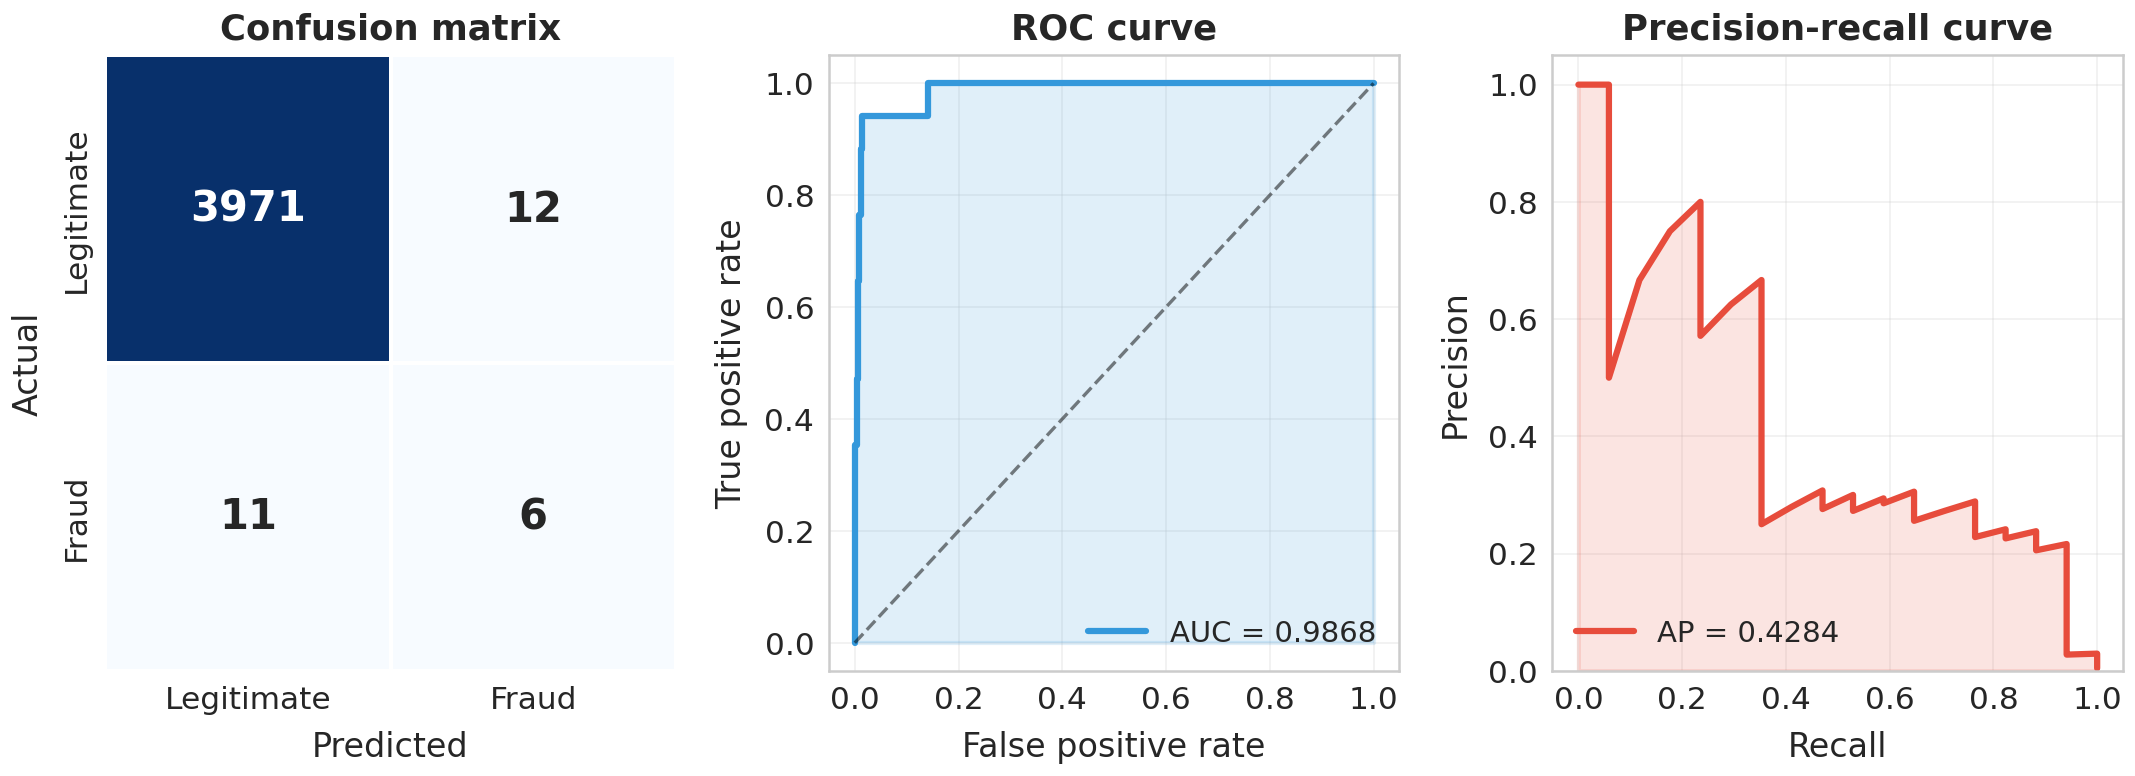
\includegraphics[width=\textwidth]{isolation_forest_eval.png}
    \caption{Isolation Forest evaluation. Left: confusion matrix reflecting conservative anomaly detection; center: ROC curve (AUC = 0.987); right: precision--recall curve (AP = 0.428).}
    \label{fig:iso_eval}
\end{figure*}

\subsubsection{XGBoost}

XGBoost achieved the best result on every metric, with a ROC-AUC and Average Precision of 1.000, an accuracy of 0.9998, and an F1-Score of 0.971. The confusion matrix (Fig.~\ref{fig:xgb_eval}) shows that all 17 fraudulent transactions were identified (zero false negatives) at the price of a single false positive among 3,983 legitimate transactions. The combination of second-order gradient boosting, shrinkage, regularized leaf weights, and the positive-class weight enables the model to concentrate on the rare, hard-to-separate fraudulent cases, which is consistent with the documented strength of XGBoost on tabular classification tasks \cite{chen2016xgboost} and with the observation that boosted and bagged ensembles dominate comparative fraud detection benchmarks \cite{sadgali2019performance,trivedi2020study}.

\begin{figure*}[!t]
    \centering
    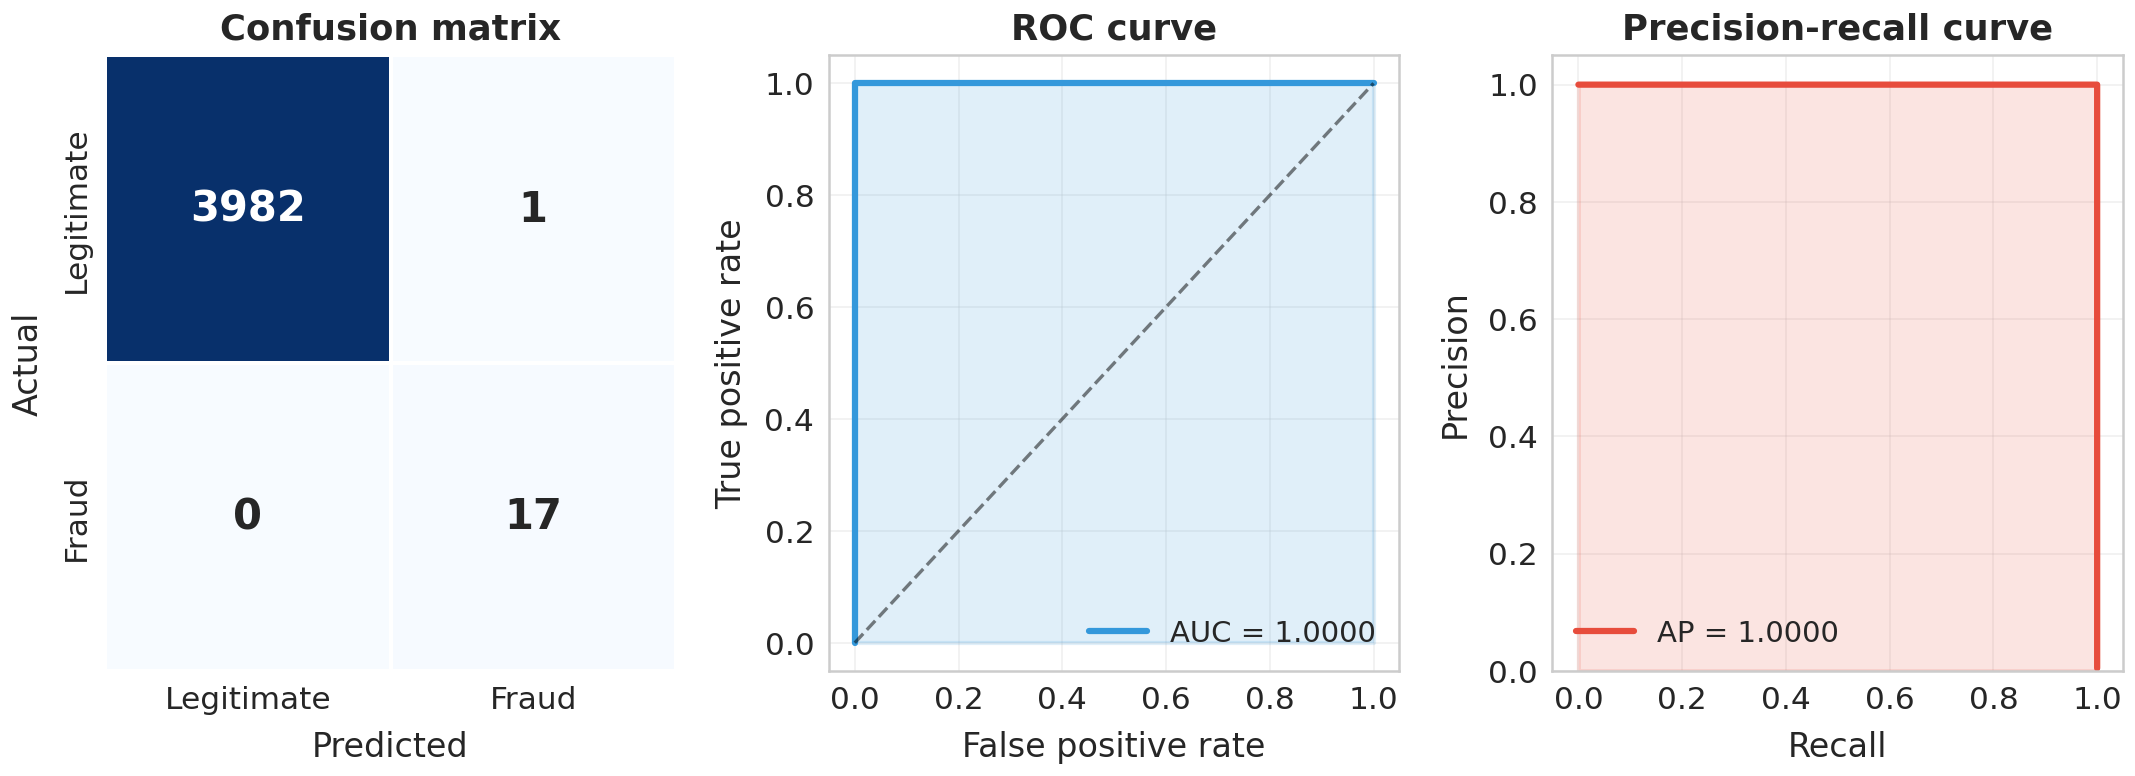
\includegraphics[width=\textwidth]{xgboost_eval.png}
    \caption{XGBoost evaluation. Left: confusion matrix with only one false positive; center: ROC curve (AUC = 1.000); right: precision--recall curve (AP = 1.000).}
    \label{fig:xgb_eval}
\end{figure*}

\subsubsection{Fraud Detection Algorithm Comparison}

Fig.~\ref{fig:fraud_comparison} presents the combined ROC curves and the metric comparison for all four algorithms. Ensemble methods occupy the top positions: XGBoost and Random Forest lead the F1-Score and Average Precision, followed at a large distance by Logistic Regression and Isolation Forest. The comparison also shows the importance of metric choice. The four ROC-AUC values lie within 0.987 and 1.000 and hardly separate the algorithms, whereas the F1-Score (0.343 to 0.971) and Average Precision (0.428 to 1.000) spread widely, in agreement with the recommendation to prefer precision--recall based measures for rare positives \cite{saito2015precision}. In a production setting, the cost of an undetected fraud typically exceeds the cost of reviewing a false alarm, so recall must be prioritized, but the review capacity of analysts sets an upper bound on the tolerable false positives. Within this trade-off, XGBoost combines full recall with only one false alarm, Random Forest provides a slightly more conservative alternative with an interpretable importance ranking, Logistic Regression secures full recall only at 54 false alarms, and Isolation Forest misses more than half of the frauds.

\begin{figure*}[!t]
    \centering
    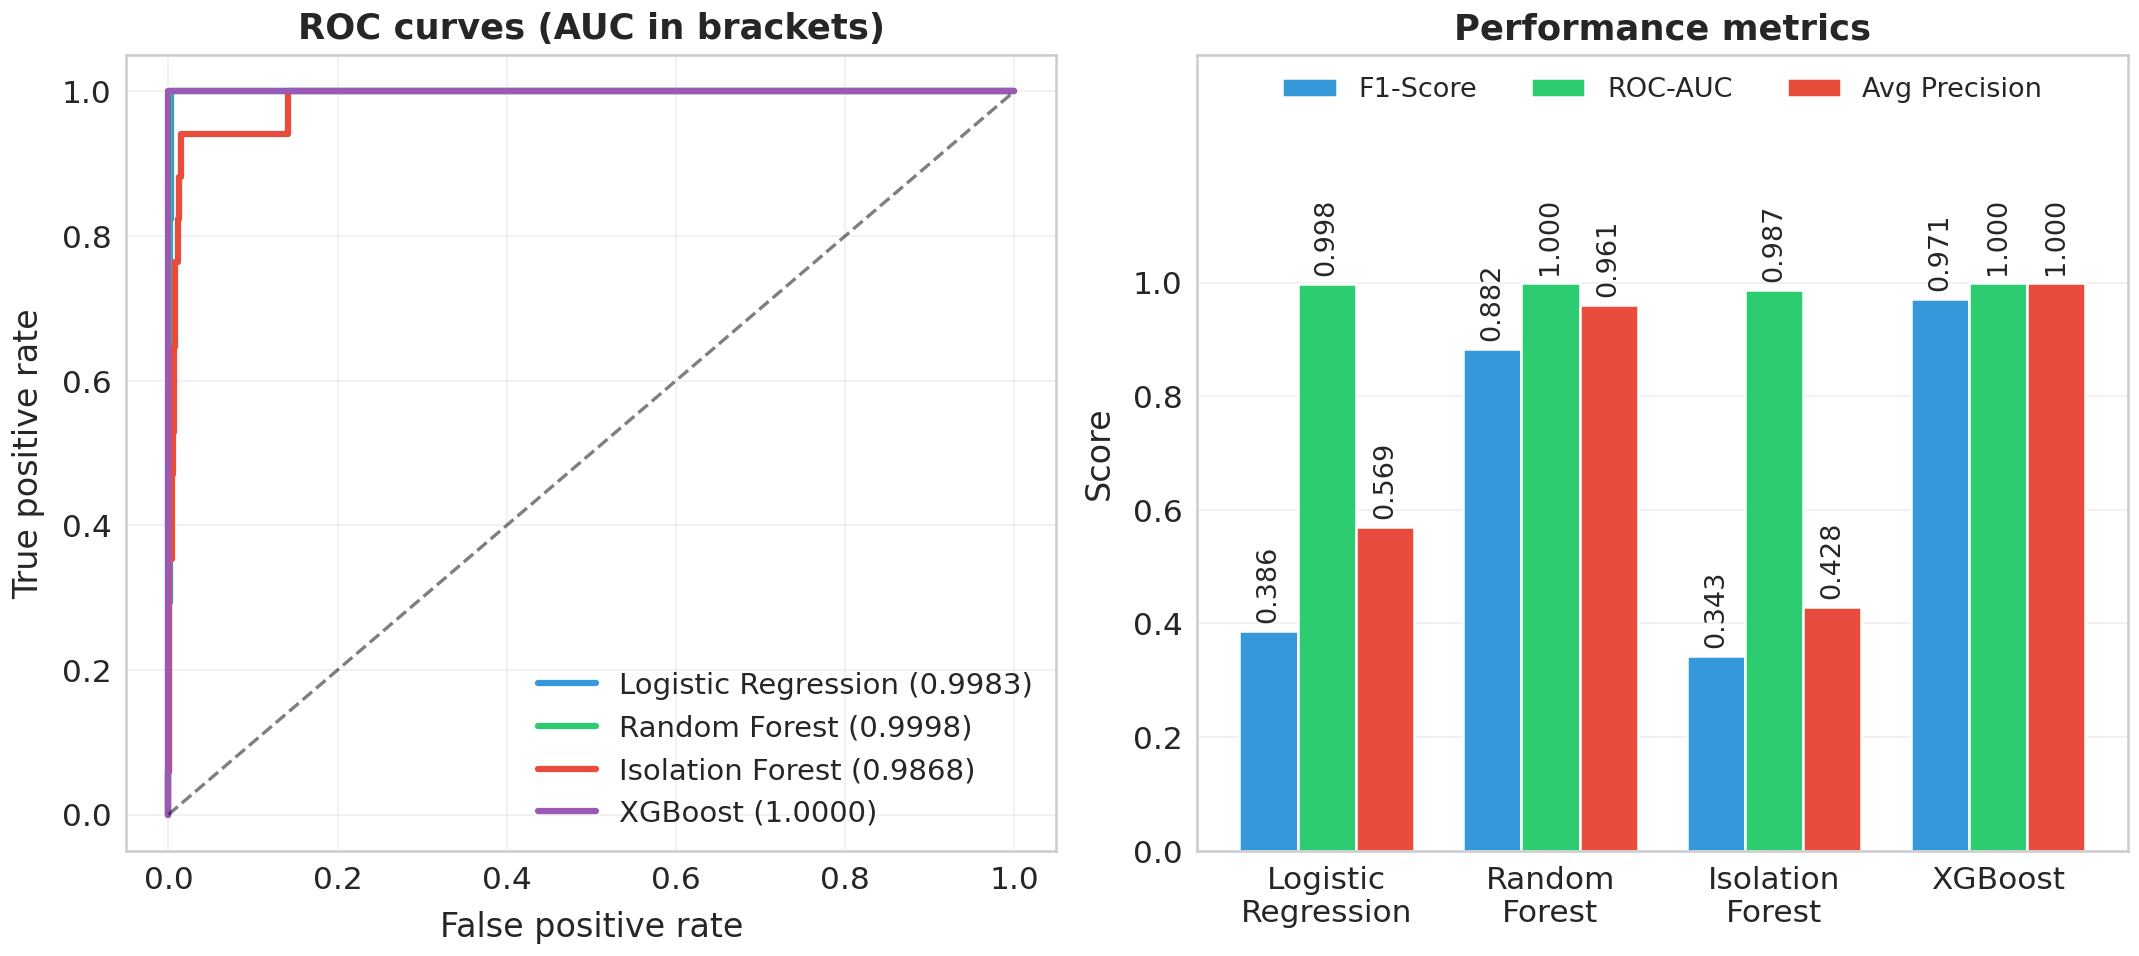
\includegraphics[width=\textwidth]{fraud_comparison_all.png}
    \caption{Fraud detection comparison. Left: ROC curves of all algorithms with AUC values in the legend; right: F1-Score, ROC-AUC, and Average Precision of each algorithm.}
    \label{fig:fraud_comparison}
\end{figure*}

The statistical reliability of these results is limited by the small number of positives. Exact 95\% Clopper--Pearson intervals for recall are [0.805, 1.000] for XGBoost and Logistic Regression (17 of 17), [0.636, 0.985] for Random Forest (15 of 17), and [0.142, 0.617] for Isolation Forest (6 of 17). The intervals of XGBoost and Random Forest overlap, so the superiority of XGBoost over Random Forest cannot be considered statistically established by a single split with 17 positives, although both models are clearly separated from Logistic Regression in precision and from Isolation Forest in recall. One additional false positive would reduce the precision of XGBoost to 0.895 and its F1-Score to 0.944, which illustrates how strongly single transactions influence the reported values.

\subsection{Cross-Task Observations}

Several observations emerge from considering the two tasks together. First, preprocessing choices affect both pipelines. Standardization and outlier capping are indispensable for distance-based clustering of skewed monetary variables, and fitting the scaler on the training partition only is indispensable for leakage-free fraud evaluation. Second, a single metric can mislead in both tasks: the Silhouette Score favored the degenerate DBSCAN partition, and accuracy and even ROC-AUC masked the false alarm problem of Logistic Regression. Reporting several complementary indices and examining cluster sizes and confusion matrices is therefore necessary. Third, the algorithms that were preferred in both tasks, K-Means and XGBoost, are scalable and have mature implementations, which matters for banks that must process millions of customers and transactions \cite{carcillo2018beyond}. Finally, the two pipelines are complementary in operation: the segments describe how customers usually behave, whereas the fraud detector flags deviations from expected behavior, and the cash-advance-reliant segment of Table~\ref{tab:profiles} and the DBSCAN noise customers are natural candidates for enhanced monitoring. The datasets used in this study are not linked at the customer level, so such an integration cannot be tested here.

\subsection{Overall Summary}

Fig.~\ref{fig:overall} presents a consolidated view of both tasks, highlighting K-Means as the recommended segmentation algorithm and XGBoost as the most effective fraud detector in these experiments. The recommendation for segmentation rests on the combination of the highest Calinski-Harabasz Index, a competitive Silhouette Score, and interpretable segments of useful size, and the recommendation for fraud detection rests on the highest F1-Score and Average Precision with full recall, with Random Forest as a robust and more transparent alternative.

\begin{figure*}[!t]
    \centering
    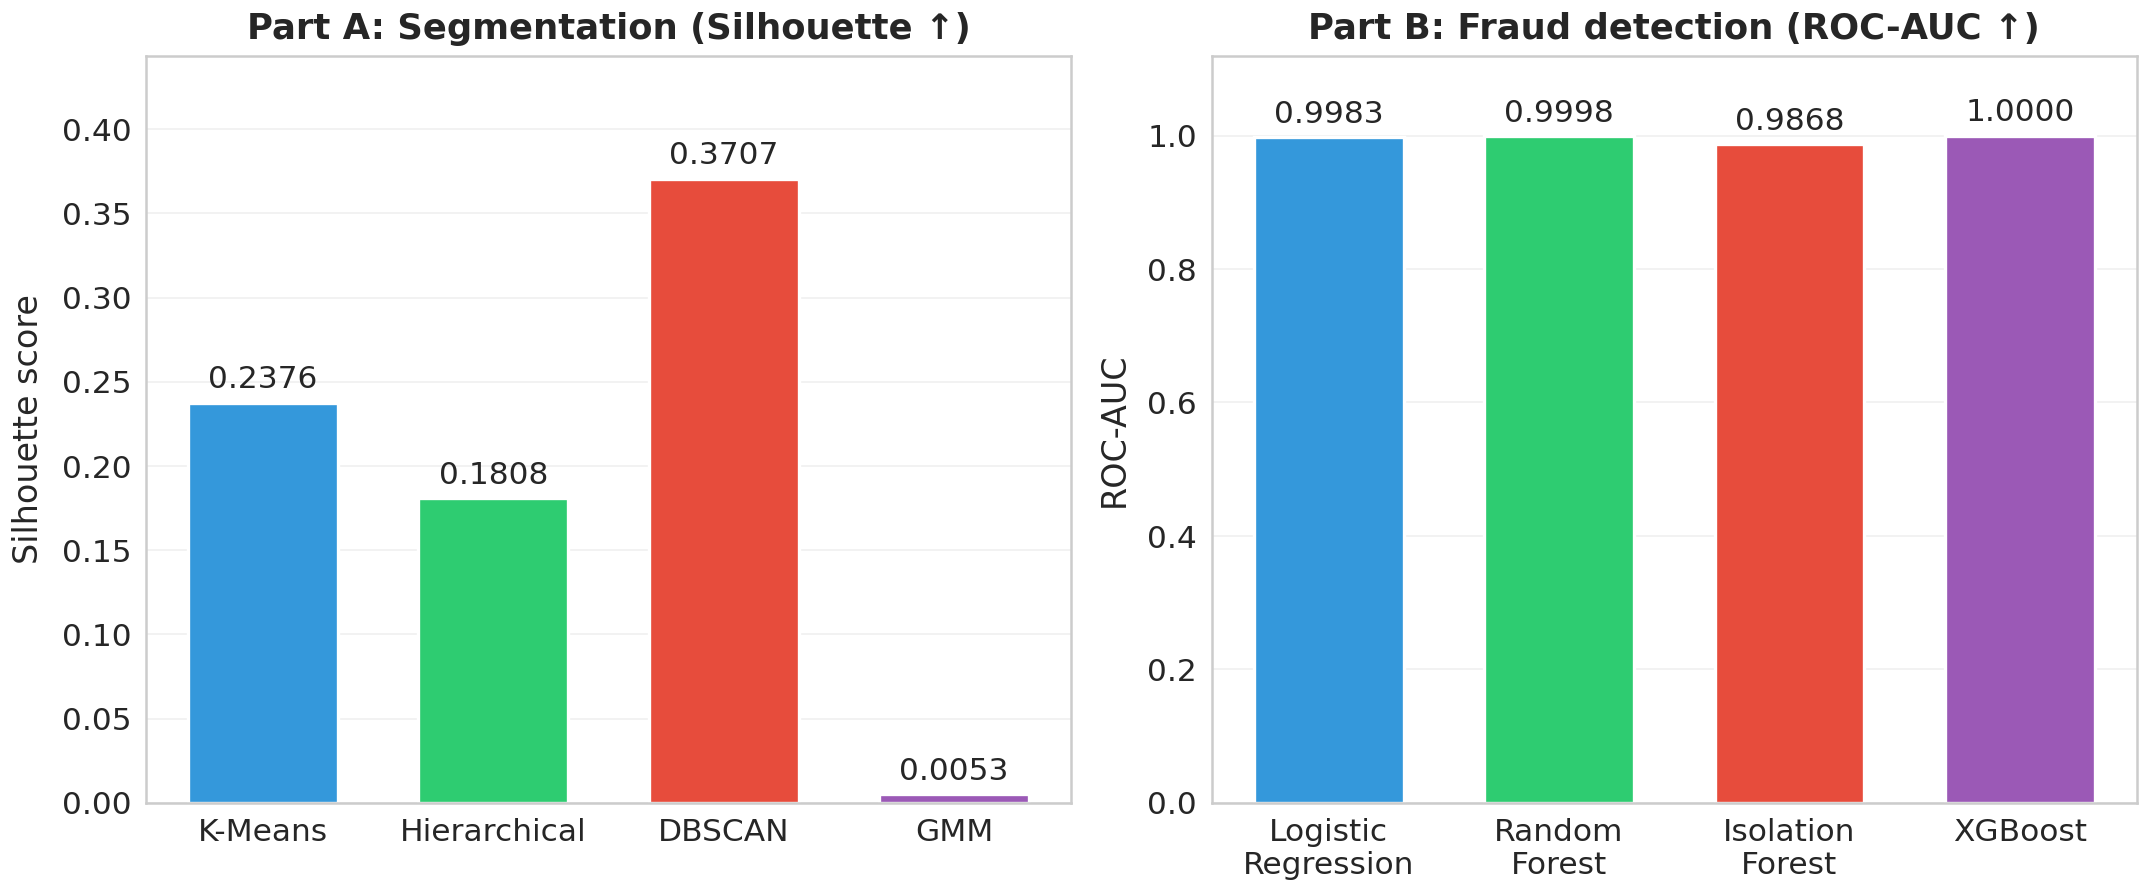
\includegraphics[width=\textwidth]{overall_project_summary.png}
    \caption{Overall results. Left: Silhouette Scores of the four segmentation algorithms; right: ROC-AUC of the four fraud detection algorithms.}
    \label{fig:overall}
\end{figure*}

\subsection{Limitations and Threats to Validity}

Several limitations should be acknowledged in interpreting the results. The fraud experiments use the first 20,000 transactions of the dataset, which cover about 8.5 hours of the first day, and the split between training and test data is random and stratified within this window, whereas production systems are evaluated forward in time and are exposed to concept drift \cite{carcillo2018beyond}; the reported performance is therefore likely to be optimistic relative to deployment. The test set contains only 17 fraudulent transactions, so that the metrics have wide confidence intervals, and single borderline predictions can change the ranking of close competitors. The PCA-transformed features of D2 prevent the economic interpretation of the detected fraud patterns. For segmentation, no ground-truth segments exist, so that only internal validity indices are available, and these indices are known to favor particular cluster shapes. The DBSCAN indices exclude noise points, the GMM search was truncated at ten components, and the hyperparameters of all models were selected by grid search over small ranges without nested cross-validation. Dataset~3 was not used in the experiments, and deep learning, sequence-based, and embedding approaches \cite{barkhordar2021,mousaeirad2020} were outside the scope of the comparison.

% ============================================================================
%  V. CONCLUSION AND FUTURE WORK
% ============================================================================
\section{Conclusion and Future Work}
\label{sec:conclusion}

This paper presented a comparative study of eight data mining algorithms applied to two banking problems, customer segmentation and fraud detection, using public credit card datasets. Four unsupervised clustering algorithms were evaluated on 8,950 customers described by 17 behavioral variables, and four supervised and anomaly detection algorithms were evaluated on a 20,000-transaction subset of the European credit card fraud dataset.

For customer segmentation, K-Means with $k=3$ provided the best balance between cluster quality (Silhouette Score of 0.2376 and Calinski-Harabasz Index of 2846.26) and practical utility. It produced three interpretable personas: high-value active spenders (22.8\%), moderate low-engagement users (51.5\%), and cash-advance-reliant revolvers (25.7\%). DBSCAN reached the highest Silhouette Score and the lowest Davies-Bouldin Index, but its partition consisted of one dominant cluster, a 32-customer satellite group, and 727 noise customers, so that its value lies in outlier screening and not in segmentation. Ward-linkage hierarchical clustering was qualitatively similar to K-Means but less compact, and the Gaussian mixture model, whose BIC kept improving up to the limit of the search range, was the weakest segmentation device.

For fraud detection, XGBoost obtained the best performance with an F1-Score of 0.971, a recall of 1.000, a ROC-AUC of 1.000, and a single false positive, followed by Random Forest with an F1-Score of 0.882. Logistic Regression secured full recall at the cost of 54 false alarms, and Isolation Forest, which uses no labels, detected 6 of 17 frauds while retaining a ROC-AUC of 0.987. Ensemble learners therefore outperformed the linear and unsupervised approaches, although the small number of test-set frauds implies wide uncertainty in these estimates. For production banking systems, K-Means is recommended for customer segmentation and XGBoost for fraud detection, with DBSCAN as an auxiliary outlier detector and Random Forest as a more transparent fallback for fraud scoring.

Future work includes validating the findings on the complete fraud dataset with time-ordered splits and repeated cross-validation, incorporating deep learning models such as autoencoders and sequence models for both tasks, adapting the fraud models to concept drift in streaming settings, implementing federated learning for privacy-preserving training across banks, conducting cost-sensitive analysis to quantify the financial impact of algorithm selection, and linking segment membership to fraud scoring when customer-level data are available.

% ============================================================================
%  ACKNOWLEDGMENT
% ============================================================================
\section*{Acknowledgment}

The authors thank the Kaggle and UCI Machine Learning Repository communities for providing open-access datasets. Special thanks to the Machine Learning Group of Universit\'{e} Libre de Bruxelles (ULB) for the European credit card fraud dataset.

% ============================================================================
%  REFERENCES
% ============================================================================
\begin{thebibliography}{99}

\bibitem{nilson2023}
The Nilson Report, ``Card fraud losses worldwide in 2023,'' \textit{The Nilson Report}, Issue 1276, Dec. 2024.

\bibitem{ngai2011application}
E. W. T. Ngai, L. Xiu, and D. C. K. Chau, ``Application of data mining techniques in customer relationship management: A literature review and classification,'' \textit{Expert Systems with Applications}, vol. 36, no. 2, pp. 2592--2602, 2009.

\bibitem{han2011data}
J. Han, M. Kamber, and J. Pei, \textit{Data Mining: Concepts and Techniques}, 3rd ed. Morgan Kaufmann, 2011.

\bibitem{bolton2002statistical}
R. J. Bolton and D. J. Hand, ``Statistical fraud detection: A review,'' \textit{Statistical Science}, vol. 17, no. 3, pp. 235--255, 2002.

\bibitem{das2022}
S. Das and J. Nayak, ``Customer segmentation via data mining techniques: State-of-the-art review,'' in \textit{Computational Intelligence in Data Mining}. Springer, 2022.

\bibitem{gomes2023}
M. Alves Gomes and T. Meisen, ``A review on customer segmentation methods for personalized customer targeting in e-commerce use cases,'' \textit{Information Systems and e-Business Management}, vol. 21, pp. 527--570, 2023.

\bibitem{hasheminejad2018}
S. M. H. Hasheminejad and M. Khorrami, ``Data mining techniques for analyzing bank customers: A survey,'' \textit{Intelligent Decision Technologies}, 2018, doi: 10.3233/IDT-180335.

\bibitem{kumar2012}
M. Varun Kumar, M. Vishnu Chaitanya, and M. Madhavan, ``Segmenting the banking market strategy by clustering,'' \textit{International Journal of Computer Applications}, vol. 45, no. 17, May 2012.

\bibitem{fouladifar2016}
A. Fouladifar, E. Taghipour, and A. Hedayati, ``Market segmentation for marketing of banking industry products: Constructing a clustering model for Bank Pasargad's e-banking customers using RFM technique and K-Means algorithm,'' \textit{International Business Management}, vol. 10, no. 6, pp. 1106--1119, 2016.

\bibitem{aryuni2018}
M. Aryuni, E. D. Madyatmadja, and E. Miranda, ``Customer segmentation in XYZ Bank using K-Means and K-Medoids clustering,'' in \textit{Proc. Int. Conf. Information Management and Technology (ICIMTech)}, Jakarta, Indonesia, 2018, pp. 412--416.

\bibitem{aliyev2020}
M. Aliyev, E. Ahmadov, H. Gadirli, A. Mammadova, and E. Alasgarov, ``Segmenting bank customers via RFM model and unsupervised machine learning,'' arXiv preprint, 2020.

\bibitem{firdaus2021}
U. Firdaus and D. N. Utama, ``Development of bank's customer segmentation model based on RFM+B approach,'' \textit{ICIC Express Letters, Part B: Applications}, vol. 12, no. 1, pp. 17--26, 2021.

\bibitem{singh2023}
K. Singh and G. Bansal, ``Customer segmentation using data mining techniques: An analysis of online retail industry,'' \textit{Juni Khyat}, vol. 13, no. 8, Aug. 2023.

\bibitem{kc2026}
S. KC and P. Pandey, ``Comparison of data mining algorithms for customer segmentation in an e-commerce dataset using clustering and classification,'' Mini Project Report (COMP 482), Dept. Comput. Sci. Eng., Kathmandu University, Dhulikhel, Nepal, 2026.

\bibitem{hasugian2026}
P. S. Hasugian, A. Simangunsong, M. Manik, and H. Tarihoran, ``Customer segmentation using K-Means clustering algorithm for digital marketing strategy,'' \textit{Jurnal Armada Informatika}, vol. 10, no. 1, pp. 251--262, Jun. 2026, doi: 10.36520/jai.v10i1.320.

\bibitem{syakur2018integration}
M. A. Syakur, B. K. Khotimah, E. M. S. Rochman, and B. D. Satoto, ``Integration K-means clustering method and Elbow method for identification of the best customer profile cluster,'' \textit{IOP Conference Series: Materials Science and Engineering}, vol. 336, p. 012017, 2018.

\bibitem{gopalakrishnan2024}
K. Gopalakrishnan, ``Customer segmentation using K-Means clustering for targeted marketing in banking,'' \textit{International Journal of Artificial Intelligence and Machine Learning}, vol. 3, no. 2, pp. 89--94, 2024, doi: 10.5281/zenodo.13627403.

\bibitem{raiter2021}
O. Raiter, ``Segmentation of bank consumers for artificial intelligence marketing,'' \textit{International Journal of Contemporary Financial Issues}, vol. 1, no. 1, pp. 39--54, 2021.

\bibitem{sinap2025}
V. Sinap, ``A deep dive into customer segmentation through advanced data mining techniques,'' \textit{DEU Fen ve M\"{u}hendislik Dergisi}, vol. 27, no. 80, pp. 272--283, 2025.

\bibitem{zakrzewska2005clustering}
D. Zakrzewska and D. Murlewski, ``Clustering algorithms for bank customer segmentation,'' in \textit{Proc. 5th International Conference on Intelligent Systems Design and Applications}, 2005, pp. 197--202.

\bibitem{hassan2018}
M. M. Hassan and M. Tabasum, ``Customer profiling and segmentation in retail banks using data mining techniques,'' \textit{International Journal of Advanced Research in Computer Science}, vol. 9, no. 4, Jul.--Aug. 2018, doi: 10.26483/ijarcs.v9i4.6172.

\bibitem{kikoria2020}
G. Kikoria, ``Bank customer clustering using a Ward method: Empirical analysis of Tbilisi, Georgia,'' \textit{Journal Association ``SEPIKE''}, no. 27, Jul. 2020.

\bibitem{yan2025}
X. Yan, Y. Li, F. Nie, and R. Li, ``Bank customer segmentation and marketing strategies based on improved DBSCAN algorithm,'' \textit{Applied Sciences}, vol. 15, no. 6, p. 3138, 2025, doi: 10.3390/app15063138.

\bibitem{kumar2024}
L. K. Kumar, D. Venkatesh, J. Katyayani, S. Sunkara, and K. Gowthami, ``A study on customer segmentation for banking sector through cluster analysis: Ethical implications,'' \textit{Communications on Applied Nonlinear Analysis}, vol. 31, no. 5s, 2024.

\bibitem{ganar2022}
C. Ganar and P. Hosein, ``Customer segmentation for improving marketing campaigns in the banking industry,'' Dept. Comput. Inf. Technol., Univ. of the West Indies, St. Augustine, Trinidad and Tobago, unpublished manuscript.

\bibitem{kovacs2021}
T. Kov\'{a}cs, A. Ko, and A. Asemi, ``Exploration of the investment patterns of potential retail banking customers using two-stage cluster analysis,'' \textit{Journal of Big Data}, vol. 8, art. 141, 2021.

\bibitem{swissvn2019}
``Segmentation of financial clients by attitudes and behavior: A comparison between Switzerland and Vietnam,'' \textit{International Journal of Bank Marketing}, vol. 37, 2019, doi: 10.1108/IJBM-07-2017-0141.

\bibitem{calvoporral2020}
C. Calvo-Porral and J.-P. L\'{e}vy-Mangin, ``An emotion-based segmentation of bank service customers,'' \textit{International Journal of Bank Marketing}, vol. 38, no. 7, pp. 1441--1463, 2020.

\bibitem{abbasimehr2021}
H. Abbasimehr and M. Shabani, ``A new methodology for customer behavior analysis using time series clustering: A case study on a bank's customers,'' \textit{Kybernetes}, 2021, doi: 10.1108/K-09-2018-0506.

\bibitem{barkhordar2021}
E. Barkhordar, M. H. Shirali-Shahreza, and H. R. Sadeghi, ``Clustering of bank customers using LSTM-based encoder-decoder and dynamic time warping,'' arXiv:2110.11769, 2021.

\bibitem{zand2020}
S. Khadivi Zand, ``Towards intelligent risk-based customer segmentation in banking,'' arXiv:2009.13929, 2020.

\bibitem{mousaeirad2020}
S. Mousaeirad, ``Intelligent vector-based customer segmentation in the banking industry,'' arXiv:2012.11876, 2020.

\bibitem{saxena2023}
A. Saxena, A. Singh, and M. Govindaraj, ``Analyzing customer churn in banking: A data mining framework,'' in \textit{Navigating the Present and Future: Contemporary Issues and Challenges in Management}, 2023, doi: 10.31893/multiscience.2023ss0310.

\bibitem{graham2025}
M. Graham, ``The impact of customer behavioral data mining on personalization strategies in digital banking services,'' unpublished manuscript, 2025.

\bibitem{aleskerov1997cardwatch}
E. Aleskerov, B. Freisleben, and B. Rao, ``CARDWATCH: A neural network based database mining system for credit card fraud detection,'' in \textit{Proc. IEEE/IAFE Computational Intelligence for Financial Engineering}, 1997, pp. 220--226.

\bibitem{bhattacharyya2011data}
S. Bhattacharyya, S. Jha, K. Tharakunnel, and J. C. Westland, ``Data mining for credit card fraud: A comparative study,'' \textit{Decision Support Systems}, vol. 50, no. 3, pp. 602--613, 2011.

\bibitem{sadgali2019performance}
I. Sadgali, N. Sael, and F. Benabbou, ``Performance of machine learning techniques in the detection of financial frauds,'' \textit{Procedia Computer Science}, vol. 148, pp. 45--54, 2019.

\bibitem{trivedi2020study}
N. K. Trivedi, S. Simaiya, U. K. Lilhore, and S. K. Sharma, ``An efficient credit card fraud detection model based on machine learning methods,'' \textit{International Journal of Advanced Science and Technology}, vol. 29, no. 5, pp. 3414--3424, 2020.

\bibitem{dal2014learned}
A. Dal Pozzolo, O. Caelen, R. A. Johnson, and G. Bontempi, ``Calibrating probability with undersampling for unbalanced classification,'' in \textit{Proc. IEEE Symposium on Computational Intelligence and Data Mining}, 2015, pp. 159--166.

\bibitem{carcillo2018beyond}
F. Carcillo, A. Dal Pozzolo, Y.-A. Le Borgne, O. Caelen, Y. Mazzer, and G. Bontempi, ``SCARFF: A scalable framework for streaming credit card fraud detection with Spark,'' \textit{Information Fusion}, vol. 41, pp. 182--194, 2018.

\bibitem{saito2015precision}
T. Saito and M. Rehmsmeier, ``The precision-recall plot is more informative than the ROC plot when evaluating binary classifiers on imbalanced datasets,'' \textit{PLoS ONE}, vol. 10, no. 3, p. e0118432, 2015.

\bibitem{kaggle_ccgeneral}
A. Bhasin, ``CC GENERAL credit card dataset,'' Kaggle, 2018. [Online]. Available: \url{https://www.kaggle.com/datasets/arjunbhasin2013/ccdata}

\bibitem{kaggle_fraud}
Machine Learning Group---ULB, ``Credit card fraud detection dataset,'' Kaggle, 2018. [Online]. Available: \url{https://www.kaggle.com/datasets/mlg-ulb/creditcardfraud}

\bibitem{uci_default}
I.-C. Yeh and C.-H. Lien, ``The comparisons of data mining techniques for the predictive accuracy of probability of default of credit card clients,'' \textit{Expert Systems with Applications}, vol. 36, no. 2, pp. 2473--2480, 2009.

\bibitem{ester1996density}
M. Ester, H.-P. Kriegel, J. Sander, and X. Xu, ``A density-based algorithm for discovering clusters in large spatial databases with noise,'' in \textit{Proc. KDD}, vol. 96, no. 34, pp. 226--231, 1996.

\bibitem{patel2020clustering}
E. Patel and D. S. Kushwaha, ``Clustering cloud workloads: K-Means vs Gaussian Mixture Model,'' \textit{Procedia Computer Science}, vol. 171, pp. 158--167, 2020.

\bibitem{chen2016xgboost}
T. Chen and C. Guestrin, ``XGBoost: A scalable tree boosting system,'' in \textit{Proc. 22nd ACM SIGKDD International Conference on Knowledge Discovery and Data Mining}, 2016, pp. 785--794.

\bibitem{liu2008isolation}
F. T. Liu, K. M. Ting, and Z.-H. Zhou, ``Isolation forest,'' in \textit{Proc. 8th IEEE International Conference on Data Mining}, 2008, pp. 413--422.

\bibitem{macqueen1967some}
J. MacQueen, ``Some methods for classification and analysis of multivariate observations,'' in \textit{Proc. 5th Berkeley Symposium on Mathematical Statistics and Probability}, vol. 1, pp. 281--297, 1967.

\bibitem{murtagh2012algorithms}
F. Murtagh and P. Contreras, ``Algorithms for hierarchical clustering: An overview,'' \textit{Wiley Interdisciplinary Reviews: Data Mining and Knowledge Discovery}, vol. 2, no. 1, pp. 86--97, 2012.

\bibitem{reynolds2009gaussian}
D. A. Reynolds, ``Gaussian mixture models,'' in \textit{Encyclopedia of Biometrics}, pp. 659--663, 2009.

\bibitem{hosmer2013applied}
D. W. Hosmer, S. Lemeshow, and R. X. Sturdivant, \textit{Applied Logistic Regression}, 3rd ed. Wiley, 2013.

\bibitem{breiman2001random}
L. Breiman, ``Random forests,'' \textit{Machine Learning}, vol. 45, no. 1, pp. 5--32, 2001.

\bibitem{rousseeuw1987silhouettes}
P. J. Rousseeuw, ``Silhouettes: A graphical aid to the interpretation and validation of cluster analysis,'' \textit{Journal of Computational and Applied Mathematics}, vol. 20, pp. 53--65, 1987.

\bibitem{davies1979cluster}
D. L. Davies and D. W. Bouldin, ``A cluster separation measure,'' \textit{IEEE Transactions on Pattern Analysis and Machine Intelligence}, vol. PAMI-1, no. 2, pp. 224--227, 1979.

\bibitem{calinski1974dendrite}
T. Cali\'{n}ski and J. Harabasz, ``A dendrite method for cluster analysis,'' \textit{Communications in Statistics---Theory and Methods}, vol. 3, no. 1, pp. 1--27, 1974.

\end{thebibliography}

\end{document}
